\subsection{用关系来解释平坦性}

在本目中，A 表示一个环，E 表示一个右 A-模，F 表示一个左 A-模。

\(\mathbf{E} \otimes_{\mathbf{A}} \mathbf{F}\) 的每个元素都至少可以用一种方式写成 \(z = \sum_{i=1}^{n} e_i \otimes f_i\) 的形式，其中 \(e_i \in \mathbf{E}\) ， \(f_i \in \mathbf{F}\) 。下面的引理给出使这个和为零的一个条件：

引理 10. 设 \((f_{\lambda})_{\lambda \in \mathbf{L}}\) 是 \(\mathbf{F}\) 的一个生成元族， \((e_{\lambda})_{\lambda \in \mathbf{L}}\) 是 \(\mathbf{E}\) 的一个支集有限的元素族。为使 \(\sum_{\lambda \in \mathbf{L}} e_{\lambda} \otimes f_{\lambda} = 0\) ，必须且只需存在有限集 \(\mathbf{J}\) 、元素族 \((x_{j})_{j \in \mathbf{J}}\) （其元素属于 \(\mathbf{E}\) ）以及元素族 \((a_{j\lambda})\) ( \(j \in \mathbf{J}, \lambda \in \mathbf{L}\) )（其元素属于 \(\mathbf{A}\) ），它们具有下列性质：

\begin{enumerate}
\def\labelenumi{(\arabic{enumi})}
\item
  族 \((a_{j\lambda})\) 的支集有限；
\item
  \(\sum_{\lambda \in L} a_{j\lambda} f_{\lambda} = 0\) 对所有 \(j \in J\) 成立；
\item
  \(e_{\lambda} = \sum_{j\in J}x_ja_{j\lambda}\) 对所有 \(\lambda \in \mathbf{L}\) 成立。
\end{enumerate}

不严格地说，诸 \(e_{\lambda}\) 所成的组，必须是 A 中元素的某些组（它们是“诸 \(f_{\lambda}\) 之间的关系”）的以 E 为系数的线性组合。

考虑自由 A-模 \(\mathrm{A}_{s}^{(\mathrm{L})}\) 、它的典范基 \((u_{\lambda})\) 以及同态 \(g: \mathrm{A}_{s}^{(\mathrm{L})} \to \mathrm{F}\) ，它满足 \(g(u_{\lambda}) = f_{\lambda}\) （对所有 \(\lambda \in L\) ）；用 R 表示 g 的核，则（由于诸 \(f_{\lambda}\) 生成 F）有正合列

\[
\mathrm{R} \xrightarrow {i} \mathrm{A} _ {s} ^ {(L)} \xrightarrow {g} \mathrm{F} \longrightarrow 0
\]

其中 i 表示典范单射。由第 1 目的引理 1，我们导出正合列

\[
\mathrm{E} \otimes_ {\mathrm{A}} \mathrm{R} \xrightarrow {1 \otimes i} \mathrm{E} \otimes_ {\mathrm{A}} \mathrm{A} _ {s} ^ {(L)} \xrightarrow {1 \otimes g} \mathrm{E} \otimes_ {\mathrm{A}} \mathrm{F} \longrightarrow 0.\tag{13}
\]

现在， \(\mathbf{E} \otimes_{\mathbf{A}} \mathbf{A}_{s}^{(L)}\) 典范地等同于 \(\mathbf{E}^{(L)}\) ，族 \(e = (e_{\lambda}) \in \mathbf{E}^{(L)}\) 等同于 \(\sum_{\lambda \in L} e_{\lambda} \otimes u_{\lambda}\) （《代数学》第二章 §3 第 7 目命题 7 的推论 1）。为使这样的族属于 \(1_{\mathbf{E}} \otimes g\) 的核，必须且只需 \(\sum_{\lambda \in L} e_{\lambda} \otimes f_{\lambda} = 0\) 在 \(\mathbf{E} \otimes_{\mathbf{A}} \mathbf{F}\) 中成立；考虑到正合列 (13)，这等价于说 \(e\) 属于 \(1_{\mathbf{E}} \otimes i\) 的像，换言之，存在形如

\[
\sum_ {\lambda \in L} e _ {\lambda} \otimes u _ {\lambda} = \sum_ {j \in J} x _ {j} \otimes i (r _ {j})\tag{14}
\]

其中 \(x_{j} \in \mathbf{E}\) ， \(r_{j} \in \mathbf{R}\) ，且 \(\mathbf{J}\) 为有限集。写 \(i(r_{j}) = \sum_{\lambda \in \mathbf{L}} a_{j\lambda} u_{\lambda}\) ，则假设 \(r_{j} \in \mathbf{R}\) 蕴含关系 \(\sum_{\lambda \in \mathbf{L}} a_{j\lambda} f_{\lambda} = 0\) 对每个 \(j \in \mathbf{J}\) 成立；另一方面，关系式 (14) 蕴含 \(e_{\lambda} = \sum_{j \in J} x_{j} a_{j\lambda}\) 对每个 \(\lambda \in \mathbf{L}\) 成立（《代数学》第二章 §3 第 7 目命题 7 的推论 1），这就完成了证明。

命题 13. 为使 E 为 F-平坦的（第 2 目，定义 1），必须且只需满足下列条件：

\begin{enumerate}
\def\labelenumi{(\Alph{enumi})}
\setcounter{enumi}{17}
\tightlist
\item
  若 \((e_i)_{i \in I}\) 与 \((f_i)_{i \in I}\) 是 E 与 F 的元素的两个有限族，使得 \(\sum_{i \in I} e_i \otimes f_i = 0\) 在 E \(\otimes_{\mathbf{A}} \mathbf{F}\) 中成立，则存在有限集 J、元素族 \((x_j)_{j \in J}\) （其元素属于 E）与元素族 \((a_{jl})\) ( \(j \in J\) ， \(i \in I\) )（其元素属于 A），它们具有下列性质：
\end{enumerate}

\begin{enumerate}
\def\labelenumi{(\arabic{enumi})}
\item
  \(\sum_{i\in I}a_{ji}f_i = 0\) 对所有 \(j\in J\) 成立
\item
  \(e_i = \sum_{j \in J} x_j a_{ji}\) 对所有 \(i \in I\) 成立。
\end{enumerate}

假设 E 是 F-平坦的。设 \((e_{i})\) 与 \((f_{i})\) 是使 \(\sum_{i\in I}e_{i}\otimes f_{i}=0\) 在 \(E\otimes_{A}F\) 中成立的元素的有限族，并设 \(F'\) 为由诸 \(f_{i}\) 生成的 F 的子模。由于典范映射 \(E\otimes_{A}F'\to E\otimes_{A}F\) 是单射， \(\sum_{i\in I}e_{i}\otimes f_{i}=0\) 在 \(E\otimes_{A}F'\) 中同样成立，于是可对 E 与 \(F'\) 应用引理 10 ；这样便得到满足 (R) 中诸条件的族 \((x_{j})\) 与 \((a_{ji})\) 。

反之，假设条件 (R) 成立。设 \(\mathbf{F}'\) 为 \(\mathbf{F}\) 的一个子模，并设 \(y = \sum_{i\in I}e_i\otimes f_i\) 为典范映射 \(\mathbf{E}\otimes_{\mathbf{A}}\mathbf{F}'\to \mathbf{E}\otimes_{\mathbf{A}}\mathbf{F}\) 的核中一个元素。由于 (R) 成立，存在满足条件 (1) 与 (2) 的族 \((x_j)\) 与 \((a_{jl})\) 。我们断言，在 \(\mathbf{E}\otimes_{\mathbf{A}}\mathbf{F}'\) 中有

\[
y = \sum_ {i, j} x _ {j} a _ {j i} \otimes f _ {i} = \sum_ {j \in J} (x _ {j} \otimes \sum_ {i \in I} a _ {j i} f _ {i}) = 0.
\]

因而 \(\mathbf{E} \otimes_{\mathbf{A}} \mathbf{F}' \to \mathbf{E} \otimes_{\mathbf{A}} \mathbf{F}\) 是单射。

推论 1. 为使右 A-模 E 是平坦的，必须且只需下列条件成立：

(RP) 若 \((e_i)_{i\in I}\) 与 \((b_i)_{i\in I}\) 是 E 与 A 的元素的两个有限族，使得 \(\sum_{i\in I}e_i b_i = 0\) ，则存在有限集 J、元素族 \((x_j)_{j\in J}\) （其元素属于 E）与元素族 \((a_{ji})\) ( \(j\in J\) ， \(i\in I\) )（其元素属于 A），使得 \(\sum_{i\in I}a_{ji}b_i = 0\) 对所有 \(j\in J\) 成立，且 \(e_i = \sum_{j\in J}x_j a_{ji}\) 对所有 \(i\in I\) 成立。

条件 (RP) 就是命题 13 的条件 (R) 应用于模 \(\mathbf{F} = \mathbf{A}_s\) 的情形。

不严格地说，(RP) 表示：诸 \(b_{i}\) 之间每个以 E 为系数的“关系”，都是诸 \(b_{i}\) 之间以 A 为系数的“关系”的（以 E 为系数的）线性组合。

我们特别考虑 A 到环 B 的一个同态，它使 B 成为右 A-模。我们知道（第 3 目，命题 1），这等价于说该 A-模是平坦的，或等价于说它对每个左 A-模 \(A_{s}^{m}\) ( \(m \geqslant 1\) ) 是平坦的。取 E = B 与 \(F = A_{s}^{m}\) 应用命题 13 的条件 (R)，便得到下列条件：

推论 2. 为使环 B 是平坦的右 A-模，必须且只需它满足下列条件：

(RP') 每个由 B 的元素组成的解 \((y_{k})_{1\leqslant k\leqslant n}\) ，若是齐次线性方程组

\[
\sum_ {k = 1} ^ {n} y _ {k} c _ {k l} = 0 \quad (1 \leqslant i \leqslant m)\tag{15}
\]

（其系数 \(c_{kl}\) 属于 A）的解，都是线性组合

\[
y _ {k} = \sum_ {j = 1} ^ {q} b _ {j} z _ {j k} \quad (1 \leqslant k \leqslant n)\tag{16}
\]

其中系数为 \(b_{j} \in \mathbf{B}\) ，组合的对象是方程组 (15) 的解 \((z_{jk})_{1 \leqslant k \leqslant n}\) ，这些解由元素 \(z_{jk}\) （属于 \(\mathbf{A}\) ）组成。

\section{忠实平坦模}

\subsection{忠实平坦模的定义}

命题 1. 设 E 是一个右 A-模。下列四个性质等价：

\begin{enumerate}
\def\labelenumi{(\alph{enumi})}
\tightlist
\item
  为使左 A-模的序列 \(\mathbf{N}' \xrightarrow{v} \mathbf{N} \xrightarrow{w} \mathbf{N}''\) 正合，必须且只需序列
\end{enumerate}

\[
\mathrm{E} \otimes_ {\mathrm{A}} \mathrm{N} ^ {\prime} \xrightarrow {1 \otimes v} \mathrm{E} \otimes_ {\mathrm{A}} \mathrm{N} \xrightarrow {1 \otimes w} \mathrm{E} \otimes_ {\mathrm{A}} \mathrm{N} ^ {\prime \prime}
\]

为正合的。

\begin{enumerate}
\def\labelenumi{(\alph{enumi})}
\setcounter{enumi}{1}
\item
  E 是平坦的，且对每个左 A-模 N，关系 \(E \otimes_{A} N = 0\) 蕴含 N = 0。
\item
  E 是平坦的，且对左 A-模的每个同态 \(v: \mathbf{N}' \to \mathbf{N}\) ，关系 \(\mathbf{1}_{\mathbf{E}} \otimes v = 0\) 蕴含 \(v = 0\) 。
\item
  E 是平坦的，且对 A 的每个极大左理想 m， \(E \neq Em\) 。为书写简便，我们对每个左 A-模 Q 置 \(T(Q) = E \otimes_{A} Q\) ，并对左 A-模的每个同态 v 置 \(T(v) = 1_{E} \otimes v\) 。
\end{enumerate}

我们先证 (a)、(b)、(c) 的等价性。

我们证明 (a) 蕴含 (b)。若 (a) 成立，则显然 E 是平坦的（§2 第 3 目，命题 1）。另一方面，设 N 是使 T(N) = 0 的左 A-模，并考虑序列 0 → N → 0；假设 T(N) = 0 意味着序列 0 → T(N) → 0 正合。由 (a)，序列 0 → N → 0 正合，从而 N = 0。

我们证明 (b) 蕴含 (c)。假设 (b) 成立，设 \(v: \mathbf{N}' \to \mathbf{N}\) 是一个同态， \(\mathbf{I}\) 是它的像。由于 \(\mathrm{T}(v)\) 的像等同于 \(\mathrm{T}(\mathbf{I})\) （§2 第 3 目，注 2），假设 \(\mathrm{T}(v) = 0\) 蕴含 \(\mathrm{T}(\mathbf{I}) = 0\) ，从而由 (b) 得 \(\mathbf{I} = 0\) ，因此 \(v = 0\) 。

我们证明 (c) 蕴含 (a)。于是假设 (c) 成立，并考虑序列

\[
\mathrm{N} ^ {\prime} \xrightarrow {v} \mathrm{N} \xrightarrow {w} \mathrm{N} ^ {\prime \prime}\tag{1}
\]

由左 A-模的同态组成的序列以及相应的序列

\[
\mathrm{T} \left(\mathrm{N} ^ {\prime}\right) \xrightarrow {\mathrm{T} (v)} \mathrm{T} (\mathrm{N}) \xrightarrow {\mathrm{T} (w)} \mathrm{T} \left(\mathrm{N} ^ {\prime \prime}\right).\tag{2}
\]

若序列 (1) 正合，则 (2) 也正合，因为 E 是平坦的（§2 第 3 目，命题 1）。反之，若 (2) 正合，则首先有 \(\mathbf{T}(w \circ v) = \mathbf{T}(w) \circ \mathbf{T}(v) = 0\) ，故由假设得 \(w \circ v = 0\) 。置 \(\mathbf{I} = v(\mathbf{N}')\) 与 \(\mathbf{K} = \overline{w}^{-1}(0)\) ；则由上所述 I 包含于 K。考虑正合序列

\[
0 \longrightarrow \mathrm{I} \stackrel {i} {\longrightarrow} \mathrm{K} \stackrel {p} {\longrightarrow} \mathrm{K} / \mathrm{I} \longrightarrow 0
\]

其中 i 与 p 是典范映射。由于 E 平坦，序列

\[
0 \longrightarrow \mathrm{T} (\mathrm{I}) \xrightarrow {\mathrm{T} (i)} \mathrm{T} (\mathrm{K}) \xrightarrow {\mathrm{T} (p)} \mathrm{T} (\mathrm{K} / \mathrm{I}) \longrightarrow 0
\]

是正合的，换言之，T(K/I) 同构于 T(K)/T(I)，而由假设后者为 0，因为 T(I)（相应地 T(K)）等同于 T(v) 的像（相应地 T(w) 的核）（§2 第 3 目，注 2）。但关系 T(p) = 0 由假设蕴含 p = 0，故 K = I，这就证明序列 (1) 正合。

最后我们证明 (b) 与 (d) 等价。若 (b) 成立，则

\[
\mathrm{E} / \mathrm{Em} = \mathrm{E} \otimes_ {\mathbf {A}} (\mathrm{A} _ {s} / \mathfrak {m}) \neq 0
\]

因为 \(A_{s}/m \neq 0\) ；从而得到 (d)。反之，假设 (d) 成立；A 的每个左理想 \(a \neq A\) 都包含在某个极大左理想 m 中（《代数学》第一章 §8 第 7 目，定理 2），于是假设 \(E \neq Em\) 蕴含 \(E \neq Ea\) ，换言之， \(E \otimes_{A} (A_{s}/a) \neq 0\) 。这就是说，对每个单生成的左 A-模 \(N \neq 0\) ， \(T(N) \neq 0\) 。现在若 N 是任一左 A-模 \(\neq 0\) ，它包含一个单生成子模 \(N' \neq 0\) ；由于 E 平坦， \(T(N')\) 等同于 \(T(N)\) 的一个子群；我们刚才看到 \(T(N') \neq 0\) ，因此 \(T(N) \neq 0\) 。

定义 1. 若右 A-模 E 满足命题 1 的四个等价条件，则称它为忠实平坦模。

忠实平坦左 A-模可类似地定义；显然，为使左 A-模 E 是忠实平坦的，必须且只需 E 视为右 \(A^{0}\) -模时是忠实平坦的。

注. 若 E 是忠实平坦 A-模，则 E 是忠实的 A-模：因为，若元素 \(a \in A\) 使对所有 \(x \in E\) 有 xa = 0，则 A 中的位似 \(h: b \mapsto ba\) 满足 \(1_{E} \otimes h = 0\) ；于是由命题 1 的性质 (c) 得 h = 0，即由于 A 有单位元而有 a = 0。

\textbf{例子}\par

\begin{enumerate}
\def\labelenumi{(\arabic{enumi})}
\item
  由命题 1 的性质 (d) 与 §2 第 3 目命题 2，一个平坦模与一个忠实平坦模的直和是忠实平坦模。
\item
  由于 \(A_{s}\) 依命题 1 的判别准则 (d) 与 §2 第 4 目例 1 是忠实平坦的，由 (1) 推出每个不化为 0 的自由模都是忠实平坦的。另一方面，存在自由模的非零直因子（换言之，非零投射模），它们是忠实的但不是忠实平坦的（习题 2）。
\item
  设 A 是主理想整环。为使 A-模 E 是忠实平坦的，必须且只需它是无挠的，且对 A 的每个不可约元素（《代数学》第七章 §1 第 3 目）p 有 \(E \neq Ep\) ；这立即由 §2 第 4 目命题 3 与命题 1 的判别准则 (d) 得出。
\end{enumerate}

\pandocbounded{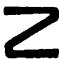
\includegraphics[keepaspectratio]{images/part001_f9c264f7.jpg}}

\begin{enumerate}
\def\labelenumi{(\arabic{enumi})}
\setcounter{enumi}{3}
\tightlist
\item
  例 (3) 表明 \(\mathbf{Z}\) -模 \(\mathbf{Q}\) 是平坦且忠实的模，但不是忠实平坦的。
\end{enumerate}

命题 2. 设 E 是忠实平坦右 A-模， \(u: \mathbf{N}' \to \mathbf{N}\) 是左 A-模同态。为使 \(u\) 是单射（相应地满射、双射），必须且只需 \(1_{\mathbf{E}} \otimes u: \mathbf{E} \otimes_{\mathbf{A}} \mathbf{N}' \to \mathbf{E} \otimes_{\mathbf{A}} \mathbf{N}\) 是如此。

这是命题 1 的判别准则 (a) 的直接推论。

命题 3. 设 \(0 \to E' \to E \to E'' \to 0\) 是右 A-模的正合列。假设 \(E'\) 与 \(E''\) 都平坦，且其中一个是忠实平坦的。则 \(E\) 是忠实平坦的。

我们已知 E 是平坦的（§2 第 5 目，命题 5）。我们验证 E 具有命题 1 的性质 (b)。设 N 是左 A-模。由于 E'' 平坦，有正合序列

\[
0 \rightarrow \mathrm{E} ^ {\prime} \otimes_ {\mathrm{A}} \mathrm{N} \rightarrow \mathrm{E} \otimes_ {\mathrm{A}} \mathrm{N} \rightarrow \mathrm{E} ^ {\prime \prime} \otimes_ {\mathrm{A}} \mathrm{N} \rightarrow 0
\]

（§2 第 5 目，命题 4）。若 \(\mathbf{E} \otimes_{\mathbf{A}} \mathbf{N} = 0\) ，则 \(\mathbf{E}' \otimes_{\mathbf{A}} \mathbf{N}\) 与 \(\mathbf{E}'' \otimes_{\mathbf{A}} \mathbf{N}\) 都为零；由于模 \(\mathbf{E}', \mathbf{E}''\) 之一是忠实平坦的，这蕴含 \(\mathbf{N} = 0\) 。

\subsection{忠实平坦模的张量积}

命题 4. 设 R、S 是两个环，E 是右 R-模，F 是 (R, S)-双模。假设 E 是忠实平坦的。则为使 F 是平坦（相应地忠实平坦）的 S-模，必须且只需 \(E \otimes_{R} F\) 是如此。

\begin{enumerate}
\def\labelenumi{(\arabic{enumi})}
\item
  若 \(\mathbf{F}\) 平坦，则 \(\mathbf{E} \otimes_{\mathbb{R}} \mathbf{F}\) 平坦（ \(\S 2\) 第 7 目，命题 8）。
\item
  假设 \(\mathbf{E} \otimes_{\mathbb{R}} \mathbf{F}\) 平坦，并设 \(v: \mathbf{N}' \to \mathbf{N}\) 是单的左 S-模同态。同态
\end{enumerate}

\[
  \mathbf {1} _ {\mathbf {E}} \otimes \mathbf {1} _ {\mathbf {F}} \otimes v: \mathbf {E} \otimes_ {\mathbf {R}} \mathbf {F} \otimes_ {\mathbf {S}} \mathbf {N} ^ {\prime} \rightarrow \mathbf {E} \otimes_ {\mathbf {R}} \mathbf {F} \otimes_ {\mathbf {S}} \mathbf {N}
\]

于是是单射（§2 第 3 目，命题 1）。由第 1 目的命题 2 推出 \(\mathbf{1}_{\mathbf{F}} \otimes v \colon \mathbf{F} \otimes_{\mathbf{S}} \mathbf{N}' \to \mathbf{F} \otimes_{\mathbf{S}} \mathbf{N}\) 是单射；于是 \(\mathbf{F}\) 是平坦的 S-模（§2 第 3 目，命题 1）。

\begin{enumerate}
\def\labelenumi{(\arabic{enumi})}
\setcounter{enumi}{2}
\item
  假设 F 是忠实平坦的，并设 N 是使 \(E \otimes_{R} F \otimes_{S} N = 0\) 的左 S-模。由于 E 是忠实平坦的，这蕴含 \(F \otimes_{S} N = 0\) ，从而由于 F 忠实平坦得 N = 0；这就证明了 \(E \otimes_{R} F\) 是忠实平坦的。
\item
  假设 \(E \otimes_{R} F\) 是忠实平坦的，并设 N 是使 \(F \otimes_{S} N = 0\) 的左 S-模。则 \(E \otimes_{R} F \otimes_{S} N = 0\) ，从而 N = 0，这表明 F 是忠实平坦的。
\end{enumerate}

推论. 设 C 是交换环，E 与 F 是两个忠实平坦 C-模。则 C-模 \(E \otimes_{C} F\) 是忠实平坦的。

取 \(\mathbf{R} = \mathbf{S} = \mathbf{C}\) 应用命题 4。

\subsection{换环}

命题 5. 设 \(\rho\) 是从环 A 到环 B 的同态。若 E 是忠实平坦右 A-模，则右 B-模 \(\rho^{*}(\mathbf{E}) = \mathbf{E}_{(\mathbf{B})} = \mathbf{E} \otimes_{\mathbf{A}} \mathbf{B}\) 是忠实平坦的。

取 R = A、S = F = B 应用第 2 目的命题 4，并注意 B-模 \(B_{d}\) 是忠实平坦的。

推论. 若 E 是忠实平坦右 A-模，且 a 是 A 的双边理想，则右 (A/a)-模 E/Ea 是忠实平坦的。

取 B = A/a 应用命题 5，其中 \(\rho\) 是典范同态。

命题 6. 设 A 是交换环，B 是 A 上的代数， \(\rho: a \mapsto a . 1\) 是 A 到 B 的典范同态。假设 B 是忠实平坦 A-模。则为使 A-模 E 是平坦（相应地忠实平坦）的，必须且只需右 B-模 \(\mathrm{E}_{(\mathrm{B})} = \mathrm{E} \otimes_{\mathrm{A}} \mathrm{B}\) 是平坦（相应地忠实平坦）的。

\begin{enumerate}
\def\labelenumi{(\arabic{enumi})}
\item
  若 E 平坦（相应地忠实平坦），则 \(E_{(B)}\) 依 §2 第 7 目命题 8 的推论 2（相应地依命题 5）是平坦（相应地忠实平坦）的。
\item
  假设 \(E_{(B)}\) 平坦，并设 \(v: N' \to N\) 是单的 A-模同态。由 §2 第 7 目推论 3，A-模 \(E \otimes_{A} B\) 平坦，因此同态 \(1_{E} \otimes 1_{B} \otimes v: E \otimes_{A} B \otimes_{A} N' \to E \otimes_{A} B \otimes_{A} N\) 是单射。由于 B 上的右与左 A-模结构一致，这个同态等同于
\end{enumerate}

\[
\mathrm{1} _ {\mathbf {E}} \otimes v \otimes \mathrm{1} _ {\mathbf {B}}: \mathrm{E} \otimes_ {\mathbf {A}} \mathrm{N} ^ {\prime} \otimes_ {\mathbf {A}} \mathrm{B} \rightarrow \mathrm{E} \otimes_ {\mathbf {A}} \mathrm{N} \otimes_ {\mathbf {A}} \mathrm{B}.
\]

由于 B 是忠实平坦 A-模，由此推出 \(1_{E} \otimes v: E \otimes_{A} N' \to E \otimes_{A} N\) 是单射（第 1 目，命题 2），这表明 E 是平坦的。

\begin{enumerate}
\def\labelenumi{(\arabic{enumi})}
\setcounter{enumi}{2}
\tightlist
\item
  最后假设 \(E_{(B)}\) 是忠实平坦的。首先由 (2)，E 是平坦的。又设 N 是使 \(E \otimes_{A} N = 0\) 的 A-模。则 \(E \otimes_{A} N \otimes_{A} B = 0\) ，于是，由于 B 上的右与左 A-模结构一致，有 \(E \otimes_{A} B \otimes_{A} N = 0\) ，它也可写成 ( \(E \otimes_{A} B\) ) \(\otimes_{B} (B \otimes_{A} N) = 0\) 。由于 \(E_{(B)}\) 是忠实平坦 B-模，这蕴含 \(B \otimes_{A} N = 0\) （第 1 目，命题 1），于是由于 B 是忠实平坦 A-模（第 1 目，命题 1）得 N = 0。
\end{enumerate}

\subsection{纯量限制}

命题 7. 设 A、B 是两个环， \(\rho\) 是 A 到 B 的同态。设 E 是忠实平坦右 B-模。为使 \(\rho^{*}(\mathrm{E})\) 是平坦（相应地忠实平坦）的右 A-模，必须且只需 B 是平坦（相应地忠实平坦）的右 A-模。

把第 2 目的命题 4 应用于以 B、A、E、B 分别代替 R、S、E、F 的情形（B 上的右 A-模结构由 \(\rho\) 定义），可以看出

B 是平坦（相应地忠实平坦）A-模，当且仅当 \(E \otimes_{B} B = \rho^{*}(E)\) 是平坦（相应地忠实平坦）A-模。

\textbf{注}\par

\begin{enumerate}
\def\labelenumi{(\arabic{enumi})}
\item
  命题 7 表明，为使 B 是忠实平坦 A-模，只需存在一个忠实平坦 B-模，它同时是忠实平坦 A-模。
\item
  设 A、B、C 是三个环， \(\rho: A \rightarrow B\) 与 \(\sigma: B \rightarrow C\) 是两个环同态。命题 7 表明：若 C 是忠实平坦 B-模且 B 是忠实平坦 A-模，则 C 是忠实平坦 A-模。若 C 是忠实平坦 B-模又是忠实平坦 A-模，则 B 是忠实平坦 A-模（为确定起见，把模都取为右模）。另一方面，B 与 C 可以都是忠实平坦 A-模而 C 不是忠实平坦 B-模（习题 7）。
\end{enumerate}

\subsection{忠实平坦环}

命题 8. 设 A、B 是两个环， \(\rho\) 是 A 到 B 的同态。假设存在右 B-模 E 使 \(\rho_{*}(E)\) 是忠实平坦 A-模。则：

\begin{enumerate}
\def\labelenumi{(\roman{enumi})}
\item
  对每个左 A-模 F，典范同态 \(j: \mathbf{F} \to \mathbf{F}_{(\mathbf{B})} = \mathbf{B} \otimes_{\mathbf{A}} \mathbf{F}\) （它满足 \(j(x) = 1 \otimes x\) ，对所有 \(x \in \mathbf{F}\) ）是单射。
\item
  对 A 的每个左理想 \(\mathfrak{a}\) ，有 \(\mathbf{A},\overline{\rho}^{-1}(\mathbf{Ba}) = \mathfrak{a}\) 。
\item
  同态 \(\rho\) 是单射。
\item
  对 A 的每个极大左理想 \(\mathfrak{m}\) ，存在 B 的极大左理想 \(\mathfrak{n}\) 使 \(\overline{\rho}^{-1}(\mathfrak{n}) = \mathfrak{m}\) 。
\end{enumerate}

我们证明 (i)。我们知道（《代数学》第二章 §5 第 2 目命题 5 的推论），对每个右 B-模 M，典范 A-同态 \(i: \mathbf{M} \to \rho_*(\mathbf{M}) \otimes_{\mathbf{A}} \mathbf{B} = \rho^*(\rho_*(\mathbf{M}))\) （由 \(i(y) = y \otimes 1\) 定义）是单射，且 A-模 \(i(\mathbf{M})\) 是 \(\rho_*(\mathbf{M}) \otimes_{\mathbf{A}} \mathbf{B}\) 的直因子。因此，对每个左 A-模 F，

\[
i \otimes 1 _ {F}: \rho_ {*} (M) \otimes_ {A} F \rightarrow \rho_ {*} (M) \otimes_ {A} B \otimes_ {A} F
\]

是单射（§2 第 1 目，引理 2）。取 \(\mathbf{M} = \mathbf{E}\) ，则（由于 \(i \otimes 1_{\mathbf{F}} = 1_{\mathbf{M}} \otimes j\) ）推出 \(j\) 是单射（第 1 目，命题 2）。

断言 (ii) 由 (i) 取 \(\mathbf{F} = \mathbf{A}_s / \mathfrak{a}\) 得出，而 (iii) 由 (ii) 取 \(\mathfrak{a} = \{0\}\) 得出。

最后，若 \(\mathfrak{m}\) 是 \(\mathbf{A}\) 的极大左理想，则由 (ii) 有 \(\bar{\rho}^{-1}(\mathbf{B}\mathfrak{m}) = \mathfrak{m}\) ，因此 \(\mathbf{B}\mathfrak{m} \neq \mathbf{B}\) 。于是存在 \(\mathfrak{n}\) ，即 \(\mathbf{B}\) 的一个包含 \(\mathbf{B}\mathfrak{m}\) 的极大左理想（《代数学》第一章 §8 第 7 目，定理 2）；这时 \(\mathfrak{m} \subset \bar{\rho}^{-1}(\mathfrak{n})\) ，且由于 \(\rho(1) \notin \mathfrak{n}\) ，有 \(1 \notin \bar{\rho}^{-1}(\mathfrak{n})\) 。因此 \(\bar{\rho}^{-1}(\mathfrak{n}) = \mathfrak{m}\) 。

若 A 与 B 满足命题 8 的条件，通常借助 \(\rho\) 把 A 等同于 B 的一个子环。

推论. 在命题 8 的假设下，若 B 是左 Noether 的（相应地左 Artin 的），则 A 亦然。

若 \((\mathfrak{a}_n)\) 是 A 的左理想组成的非稳定递增（相应地递减）序列，则 B 的理想序列 \((\mathrm{Ba}_n)\) 是非稳定且递增（相应地递减）的，因为 \(\overline{\rho}^{-1}(\mathrm{Ba}_n) = \mathfrak{a}_n\) ，这与假设相矛盾。

*注 (1). 若 A 与 B 交换，我们将在第二章 §2 第 5 目命题 11 的推论 4 中看到，命题 8 的假设蕴含

对每个 \(\text{prime}\) 理想 \(\mathfrak{p}\) （属于 \(\mathbf{A}\) ），存在 \(\text{prime}\) 理想 \(\mathfrak{q}\) （属于 \(\mathbf{B}\) ）使 \(\overline{\rho}^{-1}(\mathfrak{q}) = \mathfrak{p}\) （其中 \(\mathfrak{p} = \mathbf{A} \cap \mathfrak{q}\) ，当 \(\mathbf{A}\) 等同于 \(\mathbf{B}\) 的一个子环时）。*

命题 8 的一个重要应用是 B 本身为忠实平坦 A-模的情形。但在这种情形，我们有下面更精确的命题：

命题 9. 设 A、B 是两个环， \(\rho\) 是 A 到 B 的同态。下列五个性质等价：

\begin{enumerate}
\def\labelenumi{(\alph{enumi})}
\item
  右 A-模 B 是忠实平坦的。
\item
  同态 \(\rho\) 是单射，且右 A-模 \(\mathbf{B} / \rho (\mathbf{A})\) 是平坦的。
\item
  右 A-模 B 是平坦的，且对每个左 A-模 F，典范同态 \(x \mapsto 1 \otimes x\) （从 F 到 B \(\otimes_{A} F\) ）是单射。
\item
  右 A-模 B 是平坦的，且对 A 的每个左理想 a， \(\overline{\rho}^{-1}(\mathbf{B}\mathfrak{a}) = \mathfrak{a}\) 。
\item
  右 A-模 B 是平坦的，且对 A 的每个极大左理想 m，存在
\end{enumerate}

B 的一个极大左理想 n 使 \(\bar{\rho}^{-1}(\mathfrak{n}) = \mathfrak{m}\) 。

由命题 8，(a) 蕴含性质 (c)、(d)、(e) 中的每一个。另一方面，若 (e) 成立，则 \(\mathbf{Bm} \neq \mathbf{B}\) 对 A 的每个极大左理想 \(m\) 成立（因为存在 B 的极大左理想 \(n\) 使 \(\mathbf{Bm} \subset n\) ），且由第 1 目命题 1 的判别准则 (d)，B 是忠实平坦 A-模；因此 (e) 蕴含 (a)。

我们现在证明 \((c) \Rightarrow (d) \Rightarrow (b) \Rightarrow (a)\) ，从而完成证明。首先，在 (c) 中取 \(F = A_{s}/a\) 便知 (c) 蕴含 (d)。若 (d) 成立，取 \(a = \{0\}\) 便得 \(\rho\) 是单射；(d) 与 §2 第 6 目命题 7 的推论蕴含 \(B/\rho(A)\) 是平坦右 A-模，即 (d) 蕴含 (b)。最后，若 (b) 成立，把第 1 目的命题 3 应用于正合序列

\[
0 \longrightarrow \mathrm{A} _ {d} \stackrel {\rho} {\longrightarrow} \mathrm{B} \longrightarrow \mathrm{B} / \rho (\mathrm{A}) \longrightarrow 0
\]

由于 \(A_{d}\) 是忠实平坦的，这表明 B 是忠实平坦右 A-模。

*注 (2). 若 A 与 B 交换，我们将在第二章 §2 第 5 目命题 11 的推论 4 中看到，命题 9 的诸条件等价于下列条件：

\begin{enumerate}
\def\labelenumi{(\alph{enumi})}
\setcounter{enumi}{5}
\tightlist
\item
  B 是平坦 A-模，且对 A 的每个素理想 p，存在 B 的理想 q 使 \(\overline{\rho}^{-1}(\mathfrak{q}) = \mathfrak{p}\) 。
\end{enumerate}

在命题 9 的条件下，借助 \(\rho\) 把 A 等同于 B 的一个子环。这时关系式 \(\bar{\rho}^{-1}(\mathbf{Ba}) = a\) 就读作 \(\mathbf{A} \cap \mathbf{Ba} = a\) 。另一方面，若 F 是左 A-模，则 F 等同于它在 \(\mathbf{B} \otimes_{\mathbf{A}} \mathbf{F}\) 中的在典范映射 \(x \mapsto 1 \otimes x\) 下的像；若 X 是 F 的加法子群，我们用 BX 表示由 X 生成的 \(\mathbf{B} \otimes_{\mathbf{A}} \mathbf{F}\) 的左 B-子模。采用这个记号，我们有：

命题 10. 设 B 是环，A 是 B 的子环，且 B 是忠实平坦右 A-模。设 F 是左 A-模，F'、F'' 是 F 的两个子模。则：

\begin{enumerate}
\def\labelenumi{(\roman{enumi})}
\item
  典范映射 \(\mathbf{B} \otimes_{\mathbf{A}} \mathbf{F}' \to \mathbf{B} \otimes_{\mathbf{A}} \mathbf{F}\) 是 \(\mathbf{B} \otimes_{\mathbf{A}} \mathbf{F}'\) 到 \(\mathbf{BF}'\) 上的同构。
\item
  \(\mathbf{F} \cap \mathbf{BF}' = \mathbf{F}'\) 。
\item
  \(\mathrm{B}(\mathbf{F}' + \mathbf{F}'') = \mathbf{BF}' + \mathbf{BF}''\) 。
\item
  \(\mathbf{B}(\mathbf{F}'\cap \mathbf{F}'')=\mathbf{B}\mathbf{F}'\cap \mathbf{B}\mathbf{F}''\) 。
\end{enumerate}

由于 B 是平坦右 A-模，典范映射

\[
\mathbf {B} \otimes_ {\mathbf {A}} \mathbf {F} ^ {\prime} \rightarrow \mathbf {B} \otimes_ {\mathbf {A}} \mathbf {F}
\]

是单射；考虑到所作的等同，它的像是 BF'，这就证明了 (i)。断言 (ii) 由 §2 第 6 目命题 7 取 E = B、E' = A 并利用公式 \(A \otimes_{A} F = F\) 与 \(A \otimes_{A} F' = F'\) 得出。断言 (iii) 是平凡的，而 (iv) 由 §2 第 6 目命题 6 得出。

\subsection{忠实平坦环与有限性条件}

命题 11. 设 B 是环，A 是 B 的子环，且 B 是忠实平坦右 A-模。为使左 A-模 F 是有限生成的（相应地有限表示的），必须且只需 B-模 \(B \otimes_{A} F\) 是有限生成的（相应地有限表示的）。

\begin{enumerate}
\def\labelenumi{(\arabic{enumi})}
\item
  不对 B 作任何假设，显然，若 F 是有限生成的左 A-模，则 \(B \otimes_{A} F\) 是有限生成的左 B-模。反之，若 \(B \otimes_{A} F\) 是有限生成的 B-模，则它由形如 \(1 \otimes x_{i}\) （其中 \(x_{i} \in F\) ）的有限个元素生成；若 M 是由诸 \(x_{i}\) 生成的 F 的子 A-模，j 是典范单射 \(M \to F\) ，则 \(1_{B} \otimes j: B \otimes_{A} M \to B \otimes_{A} F\) 是满同态，于是 j 是满射（第 1 目，命题 2），这就证明 F 是有限生成的。
\item
  若 \(\mathbf{F}\) 有有限表示，则 \(\mathbf{B} \otimes_{\mathbf{A}} \mathbf{F}\) 亦然，这不需要对 B 作任何假设（§2 第 8 目）。剩下要证明：若 \(B \otimes_{A} F\) 有有限表示，则 F 亦然。我们已由 (1) 知道 F 是有限生成的，因此存在满同态 u: L → F，其中 L 是有限生成的自由 A-模。设 R 是 u 的核，则 \(B \otimes_{A} R\) 等同于满同态 \(1_{B} \otimes u: B \otimes_{A} L \to B \otimes_{A} F\) 的核（§2 第 3 目，注 2）。由于由假设 \(B \otimes_{A} F\) 有有限表示，我们断言（§2 第 8 目，引理 9） \(B \otimes_{A} R\) 是有限生成的；于是由 (1) 推出 R 是有限生成的 A-模，从而 F 有有限表示。
\end{enumerate}

命题 12. 设 B 是环，A 是 B 的中心中的交换子环，且 B 是忠实平坦 A-模。为使 A-模 F 是投射的且有限生成的，必须且只需 \(B \otimes_{A} F\) 是有限生成的投射左 B-模。

不对 A 或 B 作任何假设，这个条件显然是必要的（《代数学》第二章 §5 第 1 目命题 4 的推论）；我们证明它是充分的。由于有限生成的投射模有有限表示（§2 第 8 目，引理 8），假设蕴含 F 依命题 11 有有限表示，因此，对每个 A-模 M，有典范同构

\[
\omega : \mathbf {B} \otimes_ {\mathbf {A}} \operatorname{Hom} _ {\mathbf {A}} (\mathbf {F}, \mathbf {M}) \rightarrow \operatorname{Hom} _ {\mathbf {B}} (\mathbf {B} \otimes_ {\mathbf {A}} \mathbf {F}, \mathbf {B} \otimes_ {\mathbf {A}} \mathbf {M})
\]

（§2 第 10 目，命题 11）。然后设 \(v: \mathbf{M} \to \mathbf{M}''\) 是满的 A-模同态，并考虑交换图

\[
\begin{array}{c} \mathrm{B} \otimes_ {\mathrm{A}} \operatorname{Hom} _ {\mathrm{A}} (\mathrm{F}, \mathrm{M}) \xrightarrow {\omega} \operatorname{Hom} _ {\mathrm{B}} (\mathrm{B} \otimes_ {\mathrm{A}} \mathrm{F}, \mathrm{B} \otimes_ {\mathrm{A}} \mathrm{M}) \\ 1 _ {\mathrm{B}} \otimes \operatorname{Hom} (1 _ {\mathrm{F}}, v) \Bigg \downarrow \quad \Bigg \downarrow \operatorname{Hom} (1 _ {\mathrm{B}} \otimes \mathrm{F}, 1 _ {\mathrm{B}} \otimes v) \\ \mathrm{B} \otimes_ {\mathrm{A}} \operatorname{Hom} _ {\mathrm{A}} (\mathrm{F}, \mathrm{M} ^ {\prime \prime}) \xrightarrow [ \omega ]{\longrightarrow} \operatorname{Hom} _ {\mathrm{B}} (\mathrm{B} \otimes_ {\mathrm{A}} \mathrm{F}, \mathrm{B} \otimes_ {\mathrm{A}} \mathrm{M} ^ {\prime \prime}) \end{array}
\]

由于 \(1_{B} \otimes v\) 是满射且 \(B \otimes_{A} F\) 假设为投射的， \(\operatorname{Hom}(1_{B} \otimes F, 1_{B} \otimes v)\) 是满射（《代数学》第二章 §2 第 2 目，命题 4），因此 \(1_{B} \otimes \operatorname{Hom}(1_{F}, v)\) 也是满射。但由于 B 是忠实平坦 A-模， \(\operatorname{Hom}(1_{F}, v)\) 本身是满射（第 1 目，命题 2），因此 F 是投射 A-模（《代数学》第二章 §2 第 2 目，命题 4）。

\subsection{忠实平坦环上的线性方程组}

设 B 是环，A 是 B 的子环。若有序偶 (A, B) 满足下列条件，则称它具有线性扩张性质：

\begin{enumerate}
\def\labelenumi{(\Alph{enumi})}
\setcounter{enumi}{4}
\tightlist
\item
  线性方程组的每个由 B 的元素组成的解 \((y_{k})_{1\leqslant k\leqslant n}\) ，
\end{enumerate}

\[
\sum_ {k = 1} ^ {n} y _ {k} c _ {k \mathrm{l}} = d _ {i} \quad (1 \leqslant i \leqslant m)\tag{3}
\]

其系数 \(c_{kl}\) 与右端 \(d_{i}\) 都属于 A，它形如

\[
y _ {k} = x _ {k} + \sum_ {j = 1} ^ {p} b _ {j} z _ {j k} \quad (1 \leqslant k \leqslant n)\tag{4}
\]

其中 \((x_{k})\) 是 (3) 的由 A 的元素组成的解，诸 \(b_{j}\) 属于 B，且每个 \((z_{jk})_{1\leq k\leq n}\) 是与 (3) 相伴的齐次线性方程组的由 A 的元素组成的解。

命题 13. 设 A 是环 B 的子环。为使有序偶 (A, B) 具有线性扩张性质，必须且只需 B 是忠实平坦 A-模。

条件是充分的。因为，由于 B 是平坦 A-模，与 (3) 相伴的齐次线性方程组的每个在 B 中取值的解，都是以 B 为系数、对由 A 中元素组成的解所作的线性组合（ \(\S\) 2 第 11 目，命题 13 的推论 2）。于是问题归结为证明：若 (3) 在 B 中有解，则它在 A 中也有一个解。现在若置

\[
c _ {k} = \left(c _ {k l}\right) _ {1 \leqslant i \leqslant m} \in \mathrm{A} _ {s} ^ {m}, \quad d = (d _ {i}) \in \mathrm{A} _ {s} ^ {m},
\]

方程组 (3) 等价于方程 \(\sum_{k=1}^{n} y_k \otimes c_k = 1 \otimes d\) ，后者在 \(\mathbf{B} \otimes_{\mathbf{A}} \mathbf{A}_s^m = \mathbf{B}_s^m\) 中成立。换言之，若 \(\mathbf{M}\) 是 \(\mathbf{A}_s^m\) 的由诸 \(c_k\) ( \(1 \leqslant k \leqslant n\) ) 生成的子 A-模，则 (3) 的解 \((y_k)\) 的存在性等价于（取第 5 目中所作的等同）关系 \(d \in \mathbf{BM} \cap \mathbf{A}_s^m\) ；但由于 \(\mathbf{BM} \cap \mathbf{A}_s^m = \mathbf{M}\) （第 5 目，命题 10，(ii)），它蕴含 \(d \in \mathbf{M}\) ，即存在解 \((x_k)\) ，它由 \(\mathbf{A}\) 中元素组成，是方程组 (3) 的解。

条件是必要的。因为假设 (A, B) 具有线性扩张性质；我们已知 B 是平坦右 A-模（ \(\S\) 2 第 11 目，命题 13 的推论 2）；我们证明，对 A 的每个左理想 a， \(Ba \cap A = a\) ，这表明 B 是忠实平坦右 A-模（第 5 目，命题 9，(d)）。现在设 \(x \in Ba \cap A\) ；由假设存在 \(y_i \in B\) 与 \(a_i \in a\) 使 \(\sum_{i} y_i a_i = x\) ；把性质 (E) 应用于这个系数与右端都在 A 中的线性方程，可知存在 \(x_i \in A\) 使 \(x = \sum_{i} x_i a_i\) ，因此 \(x \in a\) 。

\section{平坦模与``Tor''函子}

为了方便熟悉同调代数 (*) 的读者，我们简要指出平坦模的理论与 Tor 函子的理论之间的联系。

命题 1. 设 E 是右 A-模。下列四个性质等价：

\begin{enumerate}
\def\labelenumi{(\alph{enumi})}
\item
  E 是平坦的。
\item
  对每个左 A-模 F 与每个整数 \(n \geqslant 1\) ， \(\operatorname{Tor}_n^{\mathbf{A}}(\mathbf{E}, \mathbf{F}) = 0\) 。
\item
  对每个左 A-模 F， \(\operatorname{Tor}_{1}^{\mathbf{A}}(\mathbf{E},\mathbf{F}) = 0\) 。
\item
  对 A 的每个有限生成左理想 a，
\end{enumerate}

\[
\operatorname{Tor} _ {1} ^ {\mathbf {A}} (\mathrm{E}, \mathrm{A} _ {s} / \mathfrak {a}) = 0.
\]

我们证明 (a) 蕴含 (b)。设

\[
\dots \rightarrow \mathrm{L} _ {n} \rightarrow \mathrm{L} _ {n - 1} \rightarrow \dots \rightarrow \mathrm{L} _ {0} \rightarrow \mathrm{F} \rightarrow 0
\]

是 F 的自由分解。由于 E 平坦，序列

\[
\dots \rightarrow \mathrm{E} \otimes \mathrm{L} _ {n} \rightarrow \mathrm{E} \otimes \mathrm{L} _ {n - 1} \rightarrow \dots \rightarrow \mathrm{E} \otimes \mathrm{L} _ {0} \rightarrow \mathrm{E} \otimes \mathrm{F} \rightarrow 0\tag{1}
\]

是正合的。由于诸 \(\operatorname{Tor}_n^{\mathbf{A}}(\mathbf{E},\mathbf{F})\) 同构于复形 (1) 的同调群，它们在 \(n\geqslant 1\) 时为零。(b) 蕴含 (c) 且 (c) 蕴含 (d) 是平凡的。最后我们证明 (d) 蕴含 (a)。正合序列

\[
0 \rightarrow a \rightarrow A _ {s} \rightarrow A _ {s} / a \rightarrow 0
\]

给出正合序列

\[
\operatorname{Tor} _ {1} ^ {\mathbf {A}} (\mathrm{E}, \mathrm{A} _ {s} / \mathfrak {a}) \rightarrow \mathrm{E} \otimes_ {\mathbf {A}} \mathfrak {a} \rightarrow \mathrm{E} \otimes_ {\mathbf {A}} \mathrm{A}.
\]

由于 (d) 成立，典范同态

\[
\mathbf {E} \otimes_ {\mathbf {A}} \mathfrak {a} \rightarrow \mathbf {E} \otimes_ {\mathbf {A}} \mathbf {A} = \mathbf {E}
\]

是单射，这就是说 E 是平坦的（§2 第 3 目，命题 1）。

命题 1 给出了平坦模的一个在应用中常常有用的判别准则。作为例子，我们只限于给出 §2 第 5 目命题 5 的一个新证明。若 E' 与 E'' 都平坦，正合序列

\[
\operatorname{Tor} _ {1} ^ {\mathbf {A}} \left(\mathrm{E} ^ {\prime}, \mathrm{F}\right)\rightarrow \operatorname{Tor} _ {1} ^ {\mathbf {A}} (\mathrm{E}, \mathrm{F}) \rightarrow \operatorname{Tor} _ {1} ^ {\mathbf {A}} \left(\mathrm{E} ^ {\prime \prime}, \mathrm{F}\right)
\]

表明 \(\operatorname{Tor}_1^{\mathbf{A}}(\mathbf{E},\mathbf{F}) = 0\) 对每个左 A-模 \(\mathbf{F}\) 成立，因此 \(\mathbf{E}\) 是平坦的。若 \(\mathbf{E}\) 与 \(\mathbf{E}''\) 都平坦，正合序列

\[
\operatorname{Tor} _ {2} ^ {\mathbf {A}} \left(\mathrm{E} ^ {\prime \prime}, \mathrm{F}\right)\rightarrow \operatorname{Tor} _ {1} ^ {\mathbf {A}} \left(\mathrm{E} ^ {\prime}, \mathrm{F}\right)\rightarrow \operatorname{Tor} _ {1} ^ {\mathbf {A}} (\mathrm{E}, \mathrm{F})
\]

表明 \(\operatorname{Tor}_1^{\mathbf{A}}(\mathbf{E}',\mathbf{F}) = 0\) ，因此 \(\mathbf{E}'\) 是平坦的。

命题 2. 设 R、S 是两个环， \(\rho: \mathbf{R} \to \mathbf{S}\) 是一个同态，F 是左 R-模。下列两个性质等价：

\begin{enumerate}
\def\labelenumi{(\alph{enumi})}
\item
  \(\operatorname{Tor}_1^{\mathbf{R}}(\rho_*(\mathbf{E}),\mathbf{F}) = 0\) ，对每个右 S-模 E。
\item
  左 S-模 \(\rho^{*}(\mathbf{F}) = \mathbf{F}_{(\mathbf{S})} = \mathbf{S} \otimes_{\mathbb{R}} \mathbf{F}\) 是平坦的，且 \(\operatorname{Tor}_{1}^{\mathbb{R}}(\rho_{*}(\mathbf{S}_{d}), \mathbf{F}) = 0\) 。
\end{enumerate}

假设 (a) 成立。取 \(E = S_{d}\) ，我们看到 \(\operatorname{Tor}_{1}^{\mathbb{R}}(\rho_{*}(S_{d}), \mathbf{F}) = 0\) 。我们还证明 \(F_{(S)}\) 是平坦 S-模。为此我们注意：若 E 是右 S-模，加法群 \(E \otimes_{S} F_{(S)}\) 等同于 \(\rho_{*}(E) \otimes_{R} F\) 。于是，若有右 S-模的正合序列

\[
0 \rightarrow \mathrm{E} ^ {\prime} \rightarrow \mathrm{E} \rightarrow \mathrm{E} ^ {\prime \prime} \rightarrow 0
\]

则利用 (a) 得到正合序列

\[
0 \rightarrow \rho_ {*} (\mathrm{E} ^ {\prime}) \otimes_ {\mathrm{R}} \mathrm{F} \rightarrow \rho_ {*} (\mathrm{E}) \otimes_ {\mathrm{R}} \mathrm{F} \rightarrow \rho_ {*} (\mathrm{E} ^ {\prime \prime}) \otimes_ {\mathrm{R}} \mathrm{F} \rightarrow 0
\]

或写作

\[
0 \rightarrow \mathrm{E} ^ {\prime} \otimes_ {\mathbf {S}} \mathrm{F} _ {(\mathbf {S})} \rightarrow \mathrm{E} \otimes_ {\mathbf {S}} \mathrm{F} _ {(\mathbf {S})} \rightarrow \mathrm{E} ^ {\prime \prime} \otimes_ {\mathbf {S}} \mathrm{F} _ {(\mathbf {S})} \rightarrow 0
\]

这就证明 \(\mathbf{F}_{(\mathbf{S})}\) 是平坦的。

反之，若 (b) 成立，首先，对每个自由右 S-模 \(L = S_{d}^{(1)}\) ，有 \(\operatorname{Tor}_{1}^{\mathrm{R}}(\rho_{*}(\mathrm{L}), \mathrm{F}) = (\operatorname{Tor}_{1}^{\mathrm{R}}(\rho_{*}(\mathrm{S}_{d}), \mathrm{F}))^{(1)} = 0\) 。每个右 S-模 E 都可写成 E = L/H 的形式，其中 L 是适当的自由 S-模；于是有正合序列

\[
0 = \operatorname{Tor} _ {1} ^ {\mathrm{R}} (\rho_ {*} (\mathrm{L}), \mathrm{F}) \rightarrow \operatorname{Tor} _ {1} ^ {\mathrm{R}} (\rho_ {*} (\mathrm{E}), \mathrm{F}) \rightarrow \rho_ {*} (\mathrm{H}) \otimes_ {\mathrm{R}} \mathrm{F} \rightarrow \rho_ {*} (\mathrm{L}) \otimes_ {\mathrm{R}} \mathrm{F}. \tag {2}
\]

但由于 \(\mathbf{F}_{(\mathbb{S})}\) 平坦，同态 \(\mathbf{H} \otimes_{\mathbb{S}} \mathbf{F}_{(\mathbb{S})} \to \mathbf{L} \otimes_{\mathbb{S}} \mathbf{F}_{(\mathbb{S})}\) 是单射，且它等同于同态

\[
\rho_ {*} (\mathrm{H}) \otimes_ {\mathbf {R}} \mathrm{F} \rightarrow \rho_ {*} (\mathrm{L}) \otimes_ {\mathbf {R}} \mathrm{F}.
\]

于是由 (2) 推出 \(\mathrm{Tor}_1^{\mathbb{R}}(\rho_*(\mathbf{E}),\mathbf{F}) = 0\) 。

注. 命题 2 也可以由下列正合序列的存在性得出

\[
\mathrm{E} \otimes_ {\mathbf {S}} \operatorname{Tor} _ {1} ^ {\mathrm{R}} (\rho_ {*} (\mathrm{S} _ {d}), \mathrm{F}) \rightarrow \operatorname{Tor} _ {1} ^ {\mathrm{R}} (\rho_ {*} (\mathrm{E}), \mathrm{F}) \rightarrow \operatorname{Tor} _ {1} ^ {\mathrm{S}} (\mathrm{E}, \mathrm{S} _ {d} \otimes_ {\mathrm{R}} \mathrm{F}) \rightarrow 0
\]

它由 Tor 函子的``结合性''谱序列导出。

\exercisesection{1}


\begin{enumerate}
\def\labelenumi{\arabic{enumi}.}
\tightlist
\item
  在交换图 (10) 中，假设有序偶 \((u', v')\) 是一个正合序列，且 \(v \circ u = 0\) 。证明
\end{enumerate}

\(\operatorname{Im}(b) \cap \operatorname{Im}(u') = b(\operatorname{Ker}(c \circ v))\) 且 \(\operatorname{Ker}(b) + \operatorname{Ker}(v) = b^{-1}(\operatorname{Im}(u' \circ a)).\)

\begin{enumerate}
\def\labelenumi{\arabic{enumi}.}
\setcounter{enumi}{1}
\tightlist
\item
  考虑交换群的交换图
\end{enumerate}

\pandocbounded{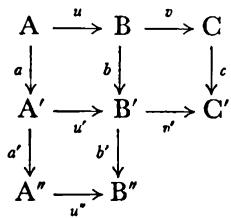
\includegraphics[keepaspectratio]{images/part001_696e1539.jpg}}

假设：(1) \((u, v)\) 与 \((b, b')\) 是正合序列；(2) \(v' \circ u' = 0\) 且 \(a' \circ a = 0\) ；(3) \(c\) 与 \(u'\) 是单射且 \(a'\) 是满射。证明在这些条件下 \(u''\) 是单射。

\begin{enumerate}
\def\labelenumi{\arabic{enumi}.}
\setcounter{enumi}{2}
\tightlist
\item
  考虑交换群的交换图
\end{enumerate}

\pandocbounded{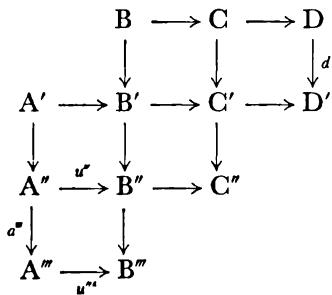
\includegraphics[keepaspectratio]{images/part001_1549be15.jpg}}

其中设各行与各列都正合，d 与 \(u''\) 是单射，\(a''\) 是满射。证明在这些条件下 \(u'''\) 是单射。推广这个结果。

\begin{enumerate}
\def\labelenumi{\arabic{enumi}.}
\setcounter{enumi}{3}
\tightlist
\item
  考虑交换群的交换图
\end{enumerate}

\pandocbounded{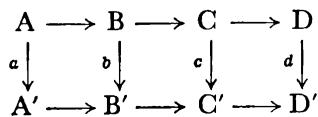
\includegraphics[keepaspectratio]{images/part001_0674edfc.jpg}}

其中设两行都是正合的。

\begin{enumerate}
\def\labelenumi{(\alph{enumi})}
\item
  证明：若 \(a\) 是满射且 \(b\) 与 \(d\) 是单射，则 \(c\) 是单射。
\item
  证明：若 \(d\) 是单射且 \(a\) 与 \(c\) 是满射，则 \(b\) 是满射。
\end{enumerate}

\begin{enumerate}
\def\labelenumi{\arabic{enumi}.}
\setcounter{enumi}{4}
\tightlist
\item
  设给定正合序列 \(A^{\prime} \xrightarrow{u} A \xrightarrow{v} A^{\prime\prime} \to 0\) 与两个满同态 \(B^{\prime} \xrightarrow{a^{\prime}} A^{\prime}, B^{\prime\prime} \xrightarrow{a^{\prime\prime}} A^{\prime\prime}\) ，其中 A, A', A'', B', B'' 是同一个环上的模。证明：若 \(B^{\prime\prime}\) 是投射模，则存在满同态 \(a: B^{\prime} \oplus B^{\prime\prime} \to A\) 使图
\end{enumerate}

\pandocbounded{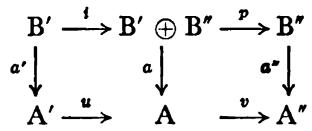
\includegraphics[keepaspectratio]{images/part001_093beead.jpg}}

是交换的（i 与 p 是典范映射）。

\begin{enumerate}
\def\labelenumi{\arabic{enumi}.}
\setcounter{enumi}{5}
\tightlist
\item
  设给定正合序列 \(0 \to A' \xrightarrow{u} A \xrightarrow{v} A''\) 与两个单同态 \(A' \xrightarrow{a'} C', A'' \xrightarrow{a''} C''\) ，其中 \(A, A', A'', C', C''\) 是同一个环上的模。证明：若 \(C'\) 是内射模（《代数学》第二章 §2 习题 11），则存在单同态 \(a: A \to C' \oplus C''\) 使图
\end{enumerate}

\pandocbounded{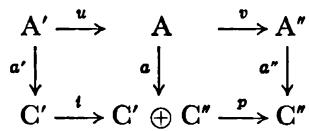
\includegraphics[keepaspectratio]{images/part001_5ee4bea9.jpg}}

是交换的（i 与 p 是典范映射）。

\begin{enumerate}
\def\labelenumi{\arabic{enumi}.}
\setcounter{enumi}{6}
\tightlist
\item
  设 U、V、W 是三个交换群， \(f: \mathrm{U} \to \mathrm{V}\) ， \(g: \mathrm{V} \to \mathrm{W}\) 是同态。
\end{enumerate}

\begin{enumerate}
\def\labelenumi{(\alph{enumi})}
\tightlist
\item
  考虑图
\end{enumerate}

\pandocbounded{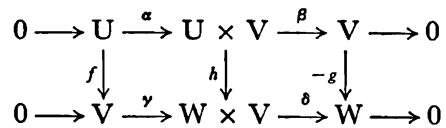
\includegraphics[keepaspectratio]{images/part001_5d67b0a0.jpg}}

其中 \(\alpha(u) = (u, f(u)), \beta(u, v) = v - f(u), \gamma(v) = (g(v), v), \delta(w, v) = w - g(v)\) ， \(h(u, v) = (g(f(u)), v)\) 。证明这个图是交换的且它的各行是正合的。

\begin{enumerate}
\def\labelenumi{(\alph{enumi})}
\setcounter{enumi}{1}
\tightlist
\item
  由 (a) 与第 4 目的命题 2 导出一个正合序列
\end{enumerate}

\[
\begin{array}{c} 0 \to \operatorname{Ker} (f) \to \operatorname{Ker} (g \circ f) \to \operatorname{Ker} (g) \to \operatorname{Coker} (f) \to \operatorname{Coker} (g \circ f) \to \\ \operatorname{Coker} (g) \to 0. \end{array}
\]

给出这个正合序列的一个直接定义。

\exercisesection{2}

\begin{enumerate}
\def\labelenumi{\arabic{enumi}.}
\item
  给出左 A-模的正合序列 \(0 \rightarrow N' \rightarrow N \rightarrow N'' \rightarrow 0\) 与右 A-模 E 的一个例子，使 E 是 \(N'\) -平坦与 \(N''\) -平坦的，但不是 N-平坦的（例如取 \(N' = N'' = Z/2Z\) ）。
\item
  设 M、N 是 A-模 E 的两个子模，且 \(M + N\) 是平坦的。为使 M 与 N 都平坦，必须且只需 \(M \cap N\) 是平坦的。
\item
  设 A 是域 K 上两个未定元的多项式环 K{[}X, Y{]} 。
\end{enumerate}

\begin{enumerate}
\def\labelenumi{(\alph{enumi})}
\item
  在 A 中考虑主理想 \(\mathfrak{b} = (\mathbf{X}), \mathfrak{c} = (\mathbf{Y})\) ，它们是自由 A-模，且其交 \(\mathfrak{b} \cap \mathfrak{c} = (\mathbf{XY})\) 也是自由的。证明 \(\mathfrak{a} = \mathfrak{b} + \mathfrak{c}\) 不是平坦 A-模，尽管 \(\mathfrak{a}\) 是无挠的（参看《代数学》第三章 §2 习题 4）。
\item
  在 A-模 \(A^{2}\) 中，设 R 是由元素 \((x, -x)\) （其中 \(x \in a\) ）组成的子模。在 A-模 \(A^{2}/R\) 中，设 M、N 是 \(A^{2}\) 的因子子模的像所成的子模；证明 M 与 N 都同构于 A，但 \(M \cap N\) 不是平坦 A-模。
\end{enumerate}

\begin{enumerate}
\def\labelenumi{\arabic{enumi}.}
\setcounter{enumi}{3}
\tightlist
\item
  \begin{enumerate}
  \def\labelenumii{(\alph{enumii})}
  \tightlist
  \item
    给出正合序列的一个例子
  \end{enumerate}
\end{enumerate}

\[
0 \rightarrow \mathrm{E} ^ {\prime} \rightarrow \mathrm{E} \rightarrow \mathrm{E} ^ {\prime \prime} \rightarrow 0
\]

它不分裂，且它的所有项都是平坦模（参看《代数学》第七章 §3 习题 8 (b)）。

\begin{enumerate}
\def\labelenumi{(\alph{enumi})}
\setcounter{enumi}{1}
\tightlist
\item
  由 (a) 导出正合序列的一个例子
\end{enumerate}

\[
0 \rightarrow \mathrm{E} ^ {\prime} \rightarrow \mathrm{E} \rightarrow \mathrm{E} ^ {\prime \prime} \rightarrow 0
\]

它不分裂，且它的各项都是非平坦的右 A-模，使得对每个左 A-模 F，序列

\[
0 \rightarrow \mathrm{E} ^ {\prime} \otimes \mathrm{F} \rightarrow \mathrm{E} \otimes \mathrm{F} \rightarrow \mathrm{E} ^ {\prime \prime} \otimes \mathrm{F} \rightarrow 0
\]

是正合的（利用第 1 目的引理 2）。

\begin{enumerate}
\def\labelenumi{\arabic{enumi}.}
\setcounter{enumi}{4}
\tightlist
\item
  给出右 A-模 E、左 A-模 F 以及 F 的两个子模 \(F'\) 、 \(F''\) 的一个例子，使 \(E \otimes (F' \cap F'')\) 在 \(E \otimes F\) 中的典范像不是 \(E \otimes F'\) 与 \(E \otimes F''\) 的典范像的交（参看习题 3(a)）。
\end{enumerate}

¶ 6. 设 A 是环，M 是左 A-模。正合序列

\[
\mathrm{L} _ {n} \rightarrow \mathrm{L} _ {n - 1} \rightarrow \dots \rightarrow \mathrm{L} _ {1} \rightarrow \mathrm{L} _ {0} \rightarrow \mathrm{M} \rightarrow 0
\]

其中 \(L_{i}\) 是自由左 A-模（ \(0 \leqslant i \leqslant n\) ），称为 M 的长度为 n 的表示或 M 的 n-表示。若所有 \(L_{i}\) 都是有限生成的自由模，则称该表示为有限表示。

若 M 是有限生成的左 A-模，用 \(\lambda(M)\) 表示一个上确界（有限的或 \(+\infty\) ），即整数 \(n \geqslant 0\) （M 对之有有限 \(n\) -表示）的上确界。若 M 不是有限生成的，则置 \(\lambda(M) = -1\) 。

\begin{enumerate}
\def\labelenumi{(\alph{enumi})}
\item
  设 \(0 \to \mathbf{P} \to \mathbf{N} \to \mathbf{M} \to 0\) 是左 A-模的正合序列。则 \(\lambda(\mathbf{N}) \geqslant \inf(\lambda(\mathbf{P}), \lambda(\mathbf{M}))\) 。（从两个 \(n\) -表示——分别属于 \(\mathbf{P}\) 与 \(\mathbf{M}\) ——出发，利用 §1 习题 5 为 \(\mathbf{N}\) 导出一个表示。）
\item
  设 \(M_{n} \xrightarrow{u_{n}} M_{n-1} \rightarrow \cdots \rightarrow M_{0} \xrightarrow{u_{0}} M \rightarrow 0\) 是 M 的有限 n-表示；证明：若 \(\lambda(M) > n\) ，则 \(\operatorname{Ker}(u_{n})\) 是有限生成的 A-模。（设
\end{enumerate}

\[
\mathrm{L} _ {n + 1} \xrightarrow {v _ {n + 1}} \mathrm{L} _ {n} \longrightarrow \dots \longrightarrow \mathrm{L} _ {2} \xrightarrow {v _ {2}} \mathrm{L} _ {1} \xrightarrow {v _ {1}} \mathrm{L} _ {0} \xrightarrow {v _ {0}} \mathrm{M} \longrightarrow 0
\]

是一个有限 \((n + 1)\) -表示——它属于 \(\mathbf{M}\) ；令 \(\mathbf{P} = \operatorname{Ker}(v_0)\) ，使存在一个 \(n\) -表示，属于 \(\mathbf{P}\) ：

\[
\mathrm{L} _ {n + 1} \xrightarrow {v _ {n + 1}} \mathrm{L} _ {n} \longrightarrow \dots \longrightarrow \mathrm{L} _ {2} \xrightarrow {v _ {2}} \mathrm{L} _ {1} \xrightarrow {v _ {1}} \mathrm{P} \longrightarrow 0.
\]

把 (a) 的方法应用于正合序列 \(0 \rightarrow P \rightarrow L_{0} \rightarrow M \rightarrow 0\) ，得到一个正合序列

\[
\mathrm{M} _ {n} \oplus \mathrm{L} _ {n + 1} \xrightarrow {w _ {n}} \mathrm{M} _ {n - 1} \oplus \mathrm{L} _ {n} \xrightarrow {w _ {n - 1}} \dots \xrightarrow {w _ {1}} \mathrm{M} _ {0} \oplus \mathrm{L} _ {1} \xrightarrow {w _ {0}} \mathrm{L} _ {0} \longrightarrow 0
\]

以及正合序列 \(0 \to \operatorname{Ker}(v_{i+1}) \to \operatorname{Ker}(w_i) \to \operatorname{Ker}(u_i) \to 0\) （§1 第 4 目，命题 2）。最后注意 \(\operatorname{Ker}(w_i)\) 是 \(\mathbf{M}_i \oplus \mathbf{L}_{i+1}\) 的直因子。

\begin{enumerate}
\def\labelenumi{(\alph{enumi})}
\setcounter{enumi}{2}
\tightlist
\item
  证明在 (a) 的假设下
\end{enumerate}

\[
\lambda (\mathbf {M}) \geqslant \inf (\lambda (\mathbf {N}), \lambda (\mathbf {P}) + 1).
\]

（若 \(n \leqslant \inf(\lambda(N), \lambda(P) + 1)\) ，则对 \(n\) 用归纳法并如 (a) 中那样论证且利用 (b)，证明 \(\lambda(M) \geqslant n\) 。）

\begin{enumerate}
\def\labelenumi{(\alph{enumi})}
\setcounter{enumi}{3}
\tightlist
\item
  证明在 (a) 的假设下
\end{enumerate}

\[
\lambda (\mathrm{P}) \geqslant \inf (\lambda (\mathrm{N}), \lambda (\mathrm{M}) - 1).
\]

（与 (c) 中方法相同。）由此推出：若 \(\lambda(N) = +\infty\) ，则 \(\lambda(M) = \lambda(P) + 1\) 。

\begin{enumerate}
\def\labelenumi{(\alph{enumi})}
\setcounter{enumi}{4}
\tightlist
\item
  由 (a)、(c) 与 (d) 推出：若 \(\mathbf{N} = \mathbf{M} \oplus \mathbf{P}\) ，则
\end{enumerate}

\[
\lambda (\mathbf {N}) = \inf (\lambda (\mathbf {M}), \lambda (\mathbf {P})).
\]

特别地，为使 N 有有限表示，必须且只需 M 与 P 也都有有限表示。

\begin{enumerate}
\def\labelenumi{(\alph{enumi})}
\setcounter{enumi}{5}
\tightlist
\item
  设 \(N_{1}\) 、 \(N_{2}\) 是 A-模 M 的两个子模。假设 \(N_{1}\) 与 \(N_{2}\) 都有有限表示。为使 \(N_{1} + N_{2}\) 有有限表示，必须且只需 \(N_{1} \cap N_{2}\) 是有限生成的。
\end{enumerate}

\begin{enumerate}
\def\labelenumi{\arabic{enumi}.}
\setcounter{enumi}{6}
\tightlist
\item
  \begin{enumerate}
  \def\labelenumii{(\alph{enumii})}
  \tightlist
  \item
    用习题 6 的记号，证明：若 M 是投射模，则 \(\lambda(M) = -1\) 或 \(\lambda(M) = +\infty\) 。若 A 是左 Noether 环，则对每个 A-模 M， \(\lambda(M) = -1\) 或 \(\lambda(M) = +\infty\) 。
  \end{enumerate}
\end{enumerate}

\begin{enumerate}
\def\labelenumi{(\alph{enumi})}
\setcounter{enumi}{1}
\item
若 \(\mathfrak{a}\) 是环 \(\mathbf{A}\) 的一个非有限生成的左理想，则 \(\mathbf{A}_s / \mathfrak{a}\) 是单生成 A-模，且不具有有限表示，换言之 \(\lambda(\mathbf{A}_s / \mathfrak{a}) = 0\) （第 8 目，引理 9）。
\item
给出环 A 的单生成左理想 \(\mathfrak{a}\) 的一个例子，使 \(\mathbf{A}_s / \mathfrak{a}\) （它有有限表示）的对偶不是有限生成的右 A-模。
\item
设 K 是交换域，E 是向量空间 \(\mathbf{K}^{(\mathbf{N})}, (e_n)\) （第二个记号是它的典范基），T 是 E 的张量代数，因此它有一个由有限乘积 \(e_{i_1}e_{i_2}\ldots e_{i_k}\) ( \(k \geqslant 0, i_j \in N\) ，对所有 j) 组成的基。对给定的整数 n，设 b 是 T 中由乘积
\end{enumerate}

\[
e _ {1} e _ {0}, e _ {2} e _ {1}, \dots , e _ {n} e _ {n - 1}
\]

与 \(e_{n+k}e_n\) （对所有 \(k\geqslant 1\) ）生成的双边理想；设 A 是商环 T/b，且对每个整数 \(m\) ，设 \(a_m\) 是 \(e_m\) 在 A 中的典范像。证明：若 \(\mathbf{M} = \mathbf{A}_s / \mathbf{A}a_0\) ，则 \(\lambda (\mathbf{M}) = n\) （注意：对 \(m\leqslant n - 1\) ， \(a_m\) 的左零化子是 \(\mathrm{A}a_{m+1}\) ，并利用习题 6(b)）。

\begin{enumerate}
\def\labelenumi{\arabic{enumi}.}
\setcounter{enumi}{7}
\item
设 C 是交换环，E、F 是两个 C-模。证明 \(\lambda(E \otimes_{\mathbb{C}} F) \geqslant \inf(\lambda(E), \lambda(F))\) 。
\item
设 E 是有限表示的左 A-模。
\end{enumerate}

\begin{enumerate}
\def\labelenumi{(\alph{enumi})}
\item
证明对右 A-模的每个族 \((\mathbf{F}_t)_{t \in I}\) ，典范同态 \(\mathbf{E} \otimes_{\mathbf{A}} \left( \prod_{t \in I} \mathbf{F}_t \right) \to \prod_{t \in I} (\mathbf{E} \otimes_{\mathbf{A}} \mathbf{F}_t)\) （《代数学》第二章 §3 第 7 目）是双射。
\item
设 \((G_{\alpha}, \phi_{\beta\alpha})\) 是左 A-模的一个归纳系；证明典范同态
\end{enumerate}

\[
\varinjlim \operatorname{Hom} _ {\mathrm{A}} (\mathrm{E}, \mathrm{G} _ {\alpha}) \rightarrow \operatorname{Hom} _ {\mathrm{A}} (\mathrm{E}, \varinjlim \mathrm{G} _ {\alpha})
\]

是双射。

\begin{enumerate}
\def\labelenumi{\arabic{enumi}.}
\setcounter{enumi}{9}
\tightlist
\item
  \begin{enumerate}
  \def\labelenumii{(\alph{enumii})}
  \tightlist
  \item
  设 A 是环，I 是集合，R 是 \(L = A_{d}^{(I)}\) 的子模。设 S 是有序偶 (J, S) 的集合，其中 J 是 I 的有限子集，S 是 \(A_{d}^{J} \cap R\) 的有限生成子模。用关系``J ⊂ J' 且 S ⊂ S'\,''给 S 排序；证明 S 关于此序关系是定向的，族 ( \(A_{d}^{J}/S\) ) 是以 S 为指标集的右 A-模的归纳系，且存在 L/R 到 \(\varinjlim (A_{d}^{J}/S)\) 上的同构。
  \end{enumerate}
\end{enumerate}

\begin{enumerate}
\def\labelenumi{(\alph{enumi})}
\setcounter{enumi}{1}
\tightlist
\item
由 (a) 推出：每个 A-模都是有限表示 A-模的归纳极限。
\end{enumerate}

\begin{enumerate}
\def\labelenumi{\arabic{enumi}.}
\setcounter{enumi}{10}
\tightlist
\item
设 E 是右 A-模。若 E 的每个有限生成子模都是有限表示的，则称 E 为伪凝聚模；伪凝聚模的每个子模都是伪凝聚的。若 E 是伪凝聚的且有限生成的（从而是有限表示的），则称 E 为凝聚模。
\end{enumerate}

\begin{enumerate}
\def\labelenumi{(\alph{enumi})}
\item
设 \(0 \to E' \to E \to E'' \to 0\) 是右 A-模的正合序列。证明：若 E 是伪凝聚（相应地凝聚）的且 \(E'\) 有限生成，则 \(E''\) 是伪凝聚（相应地凝聚）的。证明：若 \(E'\) 与 \(E''\) 都伪凝聚（相应地凝聚），则 E 亦然。证明：若 E 与 \(E''\) 都凝聚，则 \(E'\) 亦然（利用习题 6 与第 8 目的引理 9）。
\item
设 E 是凝聚 A-模， \(E'\) 是伪凝聚（相应地凝聚）A-模。证明：对每个同态 \(u: E \to E'\) ， \(\text{Im}(u)\) 与 \(\text{Ker}(u)\) 是凝聚的，且 \(\text{Coker}(u)\) 是伪凝聚（相应地凝聚）的（利用 (a)）。
\item
证明伪凝聚（相应地凝聚）模的每个直和（相应地每个有限直和）是伪凝聚（相应地凝聚）模。
\item
若 E 是伪凝聚模，M、N 是 E 的凝聚子模，证明 \(M + N\) 与 \(M \cap N\) 是凝聚的（利用 (a) 与 (c)）。
\item
假设 A 交换。证明：若 E 是凝聚 A-模且 F 是凝聚（相应地伪凝聚）A-模，则 \(\operatorname{Hom}_{\mathbf{A}}(\mathbf{E}, \mathbf{F})\) 是凝聚（相应地伪凝聚）A-模。（归结为 F 为凝聚的情形，考虑 E 的一个有限表示，然后利用 (b)。）
\end{enumerate}

¶ 12. (a) 设 A 是环。证明下列四个性质等价：

\((\alpha)\) 右 A-模 \(\mathbf{A}_d\) 是凝聚的（习题 11）。

(β) 每个有限表示的右 A-模都是凝聚的。

(γ) 每个 A-模 \(A_{s}^{I}\) （I 为任意集合）都是平坦的。

(δ) 平坦左 A-模的每个乘积都是平坦的。

（为证明 \((\alpha)\) 蕴含 \((\beta)\) ，利用习题 11(b)。为看出 \((\gamma)\) 蕴含 \((\alpha)\) ，利用第 11 目的命题 13 并用反证法论证。为证明 \((\alpha)\) 蕴含 \((\delta)\) ，利用习题 9。）

这样的环称为右凝聚环，左凝聚环的概念类似地定义。

\begin{enumerate}
\def\labelenumi{(\alph{enumi})}
\setcounter{enumi}{1}
\tightlist
\item
  证明每个右 Noether 环都是右凝聚的。给出一个不是左凝聚的右 Artin 环的例子（参看《代数学》第八章 §2 习题 4）。
\end{enumerate}

*(c) 秩 1 的非离散赋值环（第六章）是凝聚的，但它含有非凝聚的理想，并且有（单生成的）非伪凝聚的商模。*

\begin{enumerate}
\def\labelenumi{(\alph{enumi})}
\setcounter{enumi}{3}
\item
  证明：若 A 是右凝聚环，则对每个右 A-模 E， \(\lambda(\mathrm{E}) = -1\) 或 \(\lambda(\mathrm{E}) = 0\) 或 \(\lambda(\mathrm{E}) = +\infty\) （习题 6）。
\item
设 \((\mathbf{A}_{\alpha}, \phi_{\beta \alpha})\) 是环的归纳系，其指标集是定向的，且设 \(\mathbf{A} = \varinjlim \mathbf{A}_{\alpha}\) 。假设对 \(\alpha \leqslant \beta\) ， \(\mathbf{A}_{\beta}\) 是平坦右 \(\mathbf{A}_{\alpha}\) -模。证明：若诸 \(\mathbf{A}_{\alpha}\) 都右凝聚，则 \(\mathbf{A}\) 亦然。（注意 \(\mathbf{A}\) 是平坦 \(\mathbf{A}_{\alpha}\) -模（对所有 \(\alpha\) ），且若 \(\mathbf{E}\) 是 \(\mathbf{A}_d\) 的有限生成子模，则存在指标 \(\alpha\) 以及有限生成子模 \(\mathbf{E}_{\alpha}\) （属于 \((\mathbf{A}_{\alpha})_d\) ），使 \(\mathbf{E}_{\alpha} \otimes_{\mathbf{A}_{\alpha}} \mathbf{A}\) 同构于 \(\mathbf{E}\) 。）
\end{enumerate}

* (f) 由 (e) 推出：Noether 交换环上的每个多项式环（在任何有限或无限未定元集上）都是凝聚的。由此推出：凝聚环的商环未必凝聚。*

\begin{enumerate}
\def\labelenumi{(\alph{enumi})}
\setcounter{enumi}{6}
\tightlist
\item
  为使 A 左凝聚，必须且只需 A 的每个元素的左零化子是有限生成的，且 A 的两个有限生成左理想的交是有限生成的（利用习题 6(f)）。
\end{enumerate}

¶ 13. 设 A、B 是两个环，F 是 (A, B)-双模，G 是右 B-模。证明：若 G 是内射的（《代数学》第二章 §2 习题 11）且 F 是平坦左 A-模，则右 A-模 \(\operatorname{Hom}_{B}(F, G)\) 是内射的。（利用同构

\[
\operatorname{Hom} _ {\mathbf {A}} (\mathbf {E}, \operatorname{Hom} _ {\mathbf {B}} (\mathbf {F}, \mathbf {G})) \rightarrow \operatorname{Hom} _ {\mathbf {B}} (\mathbf {E} \otimes_ {\mathbf {A}} \mathbf {F}, \mathbf {G})
\]

其中 E 是右 A-模（《代数学》第二章 §4 第 1 目）。）

¶ 14. 设 A、B 是两个环，E 是左 A-模，F 是 (A, B)-双模，G 是右 B-模；考虑典范同态（《代数学》第二章 §4 习题 5）

\[
\sigma \colon \operatorname{Hom} _ {\mathbb {B}} (\mathrm{F}, \mathrm{G}) \otimes_ {\mathrm{A}} \mathrm{E} \rightarrow \operatorname{Hom} _ {\mathbb {B}} (\operatorname{Hom} _ {\mathrm{A}} (\mathrm{E}, \mathrm{F}), \mathrm{G})
\]

它满足 \((\sigma(u \otimes x))(v) = u(v(x))\) ，对所有 \(x \in \mathbf{E}\) ， \(u \in \operatorname{Hom}_{\mathbf{B}}(\mathbf{F}, \mathbf{G})\) ，

\[
v \in \operatorname{Hom} _ {\mathbf {A}} (\mathrm{E}, \mathbf {F}).
\]

证明：若 G 是内射 B-模（《代数学》第二章 §2 习题 11）且 E 有限表示，则 \(\sigma\) 是双射。（先考虑 E 是自由且有限生成的情形。）

¶ 15. 设 A 是环。证明每个平坦且有限表示的左 A-模 E 都是投射的。（给定左 A-模的满同态 \(u: \mathbf{F} \to \mathbf{F}'\) ，设 \(u'\) 是同态

\[
\operatorname{Hom} \left(1 _ {\mathbf {E}}, u\right): \operatorname{Hom} _ {\mathbf {A}} (\mathrm{E}, \mathrm{F}) \rightarrow \operatorname{Hom} _ {\mathbf {A}} (\mathrm{E}, \mathrm{F} ^ {\prime \prime})
\]

且设 \(\bar{u}\) 是同态

\[
\operatorname{Hom} \left(u ^ {\prime}, 1 _ {G}\right): \operatorname{Hom} _ {\mathbf {Z}} \left(\operatorname{Hom} _ {A} (E, F ^ {\prime \prime}), G\right)\rightarrow \operatorname{Hom} _ {\mathbf {Z}} \left(\operatorname{Hom} _ {A} (E, F), G\right),
\]

其中 G 是可除 Z-模。先利用习题 14 证明 \(\bar{u}\) 是单射；然后取适当的 G（《代数学》第二章 §2 习题 14），证明 \(u'\) 是满射。）

\begin{enumerate}
\def\labelenumi{\arabic{enumi}.}
\setcounter{enumi}{15}
\tightlist
\item
  设 A 是环， \(a\) 是 A 的元素。证明下列性质等价。
\end{enumerate}

\((\alpha)\) \(a \in aAa\) 。

(β) aA 是模 \(A_{d}\) 的直因子。

(γ) \(A_{d}/aA\) 是平坦右 A-模。

(δ) 对 A 的每个左理想 b， \(aA \cap b = ab\) 。

（利用第 6 目命题 7 的推论证明 \((\gamma)\) 与 \((\delta)\) 的等价性，并直接证明 \((\delta)\) 蕴含 \((\alpha)\) 且 \((\alpha)\) 蕴含 \((\beta)\) ，办法是证明存在幂等元 \(e \in a\mathbf{A}\) 使 \(e\mathbf{A} = a\mathbf{A}\) 。）

\begin{enumerate}
\def\labelenumi{\arabic{enumi}.}
\setcounter{enumi}{16}
\tightlist
\item
  设 A 是环。证明下列性质等价：
\end{enumerate}

(α) 每个元素 \(a \in A\) 都满足习题 16 的等价性质。

(β) A 的每个有限生成右理想都是 \(A_{d}\) 的直因子。

(γ) 每个左 A-模都是平坦的。

(δ) 每个右 A-模都是平坦的。

这时称 A 为绝对平坦环 (*)。

（为看出 \((\alpha)\) 蕴含 \((\beta)\) ，利用《代数学》第八章 §6 习题 15(b)。）

¶ 18. 设 A 是绝对平坦环（习题 17）。

\begin{enumerate}
\def\labelenumi{(\alph{enumi})}
\item
  设 P 是投射右 A-模。证明 P 的每个有限生成子模 E 都是 P 的直因子。（归结为 P 自由且有限生成的情形。然后注意 P/E 是有限表示的并利用习题 15。）
\item
  证明每个投射右 A-模 P 都是单生成子模的直和，这些子模同构于 A 的单生成右理想。（利用 Kaplansky 定理（《代数学》第二章 §2 习题 3）把问题归结为 P 由可数族元素生成的情形，然后利用 (a)。）
\item
给出绝对平坦环 A 与非投射的有限生成 A-模的一个例子（考虑 A 对一个非有限生成理想的商；参看《代数学》第八章 §6 习题 15(f) 与《交换代数》第二章 §4 习题 17）。
\end{enumerate}

\begin{enumerate}
\def\labelenumi{\arabic{enumi}.}
\setcounter{enumi}{18}
\tightlist
\item
  设 A 是环。证明下列性质等价：
\end{enumerate}

\((\alpha)\) A 是半单的。

(β) A 的每个右理想都是内射 A-模。

(γ) 每个右 A-模都是投射的。

(δ) 每个右 A-模都是内射的。

\begin{enumerate}
\def\labelenumi{\arabic{enumi}.}
\setcounter{enumi}{19}
\item
  设 A 是整环，B 是作为 A-模平坦的 A-代数，M 是无挠 A-模。证明：若 \(t \in B\) 不是零因子，则对 \(z \in B \otimes_{A} M\) 关系 t. z = 0 蕴含 z = 0。（归结为 M 有限生成的情形，且通过把 M 嵌入一个有限生成的自由 A-模，归结为 M = A 的情形。）
\item
  设 S 是交换环，R 是交换 S-代数，B 是 S-代数（交换或非交换）， \(\mathrm{B}_{(\mathrm{R})}\) 是由 B 经纯量扩张得到的 R-代数。假设 R 是平坦 S-模且 B 是有限生成 S-模。若 Z 是 B 的中心，证明从 \(Z_{(R)} = Z \otimes_{S} R\) 到 \(\mathrm{B}_{(\mathrm{R})}\) 的典范同态是 \(Z_{(R)}\) 到 \(\mathrm{B}_{(\mathrm{R})}\) 的中心上的同构。（利用正合序列
\end{enumerate}

\[
0 \longrightarrow \mathrm{Z} \longrightarrow \mathrm{B} \stackrel {\theta} {\longrightarrow} \operatorname{Hom} _ {\mathrm{s}} (\mathrm{B}, \mathrm{B})
\]

其中 \(\theta (x)(y) = xy - yx\) ，以及第 10 目的命题 11。）

\begin{enumerate}
\def\labelenumi{\arabic{enumi}.}
\setcounter{enumi}{21}
\tightlist
\item
  设 E 是左 A-模。对 A 的每个右理想 a 与每个元素 \(a \in A\) ，用 a: a 表示 \(x \in A\) （满足 \(ax \in a\) ）所成的集合，用 aE: a 表示 \(y \in E\) （满足 \(ay \in aE\) ）所成的集合。这时显然有 (a: a)E ⊂ aE: a。证明：为使 E 平坦，必须且只需对 A 的每个右理想 a 与每个元素 \(a \in A\) ，(a: a)E = aE: a。（为看出条件是必要的，考虑右 A-模的正合序列 \(0 \to (a: a)/a \stackrel{\psi}{\to} A_d/a \stackrel{\varphi}{\to} A_d/a\) ，其中 \(\psi\) 是典范单射， \(\phi\) 是由用 a 左乘再取商得到的映射。为看出条件是充分的，应用第 11 目命题 13 的推论 1 的判别准则：从一个关系 \(\sum_{i=1}^{n} a_i x_i = 0\) 出发，其中 \(a_i \in A\) ， \(x_i \in E\) ，把假设应用于理想
\end{enumerate}

\(a_{2}=\sum_{i=2}^{n}a_{i}A\) 与元素 \(a_{1}\) ，并对 n 用归纳法论证。）

\begin{enumerate}
\def\labelenumi{\arabic{enumi}.}
\setcounter{enumi}{22}
\tightlist
\item
  \begin{enumerate}
  \def\labelenumii{(\alph{enumii})}
  \tightlist
  \item
  设 \(0 \to \mathbf{R} \to \mathbf{L} \to \mathbf{E} \to 0\) 是左 A-模的正合序列，其中 \(\mathbf{L}\) 是自由 A-模；设 \((e_{\alpha})\) 是 \(\mathbf{L}\) 的基。证明下列条件等价：
  \end{enumerate}
\end{enumerate}

(α) E 是平坦的。

(β) 对所有 \(x \in \mathbb{R}\) ，若 \(\mathfrak{a}_x\) 是 \(x\) 关于基 \((e_{\alpha})\) 的分量生成的右理想，则 \(x \in \mathbb{R}\mathfrak{a}_x\) 。

\((\gamma)\) 对所有 \(x \in \mathbb{R}\) ，存在同态 \(u_x: \mathbf{L} \to \mathbf{R}\) 使 \(u_x(x) = x\) 。

\begin{enumerate}
\def\labelenumi{(\arabic{enumi})}
\setcounter{enumi}{7}
\tightlist
\item
对 R 中元素的每个有限序列 \((x_{i})_{1\leqslant i\leqslant n}\) ，存在同态 \(u\colon \mathbf{L}\to \mathbb{R}\) 使 \(u(x_{i}) = x_{i}\) （对 \(1\leqslant i\leqslant n\) ）。（利用第 6 目命题 7 的推论。）
\end{enumerate}

\begin{enumerate}
\def\labelenumi{(\alph{enumi})}
\setcounter{enumi}{1}
\tightlist
\item
  设 \(\mathfrak{a}\) 是 \(\mathbf{A}\) 的左理想，使 \(\mathbf{A} / \mathfrak{a}\) 是平坦 \(\mathbf{A}\) -模。证明：对每个有限生成左理想 \(\mathfrak{b} \subset \mathfrak{a}\) ，存在 \(x \in \mathbf{A}\) 使
\end{enumerate}

\[
\mathfrak {b} \subset \mathrm{A} x \subset \mathfrak {a}
\]

（利用 (a) 的条件 (δ)）。

\begin{enumerate}
\def\labelenumi{(\alph{enumi})}
\setcounter{enumi}{2}
\item
  由 (a) 导出习题 15 的结果的一个新证明。
\item
  设 \(\mathfrak{r}\) 是 \(\mathbf{A}\) 的 Jacobson 根，且 \(0 \to \mathbf{R} \to \mathbf{L} \to \mathbf{E} \to 0\) 是左 A-模的正合序列，其中 \(\mathbf{L}\) 是自由的。假设 \(\mathbf{E}\) 平坦且 \(\mathbf{R}\) 包含于 \(\mathfrak{rL}\) 。证明 \(\mathbf{R} = 0\) （用 (a) 的记号，注意 \(\mathfrak{a}_x\) 是有限生成理想且 \(\mathfrak{a}_x = \mathfrak{a}_x\mathfrak{r}\) ）。
\item
  设 E 是有限生成的平坦 A-模；假设存在 A 的包含于 Jacobson 根中的双边理想 b，使 E/bE 是自由 (A/b)-模。证明这时 E 是自由 A-模（注意存在有限生成自由 A-模 L 使 L/bL 同构于 E/bE，并利用《代数学》第八章 §6 第 3 目命题 6 的推论 4；然后应用 (d)）。
\end{enumerate}

\begin{enumerate}
\def\labelenumi{\arabic{enumi}.}
\setcounter{enumi}{23}
\tightlist
\item
右 A-模 M 的子模 \(M'\) 称为纯的，如果用 \(j: M' \rightarrow M\) 表示典范单射，同态
\end{enumerate}

\[
j \otimes 1 _ {N} \colon M ^ {\prime} \otimes_ {A} N \rightarrow M \otimes_ {A} N
\]

对每个左 A-模 N 是单射。若 \(M'\) 是 M 的直因子或 \(M/M'\) 平坦，情形就是如此，但这两个条件不是必要的（习题 4）。

\begin{enumerate}
\def\labelenumi{(\alph{enumi})}
\item
  证明：为使 \(\mathbf{M}'\) 是 \(\mathbf{M}\) 的纯子模，必须且只需：若 \((m_i')_{i\in I}\) 是 \(\mathbf{M}'\) 的元素的有限族， \((x_j)_{j\in J}\) 是 \(\mathbf{M}\) 的元素的族，使 \(m_i' = \sum_{j\in J} x_j a_{jl}\) 对所有 \(i\in I\) 成立，且 \((a_{jl})\) 是 \(\mathbf{A}\) 的元素的族，则存在族 \((x_j')_{j\in J}\) （元素属于 \(\mathbf{M}'\) ）使 \(m_i' = \sum_{j\in J} x_j' a_{jl}\) 对所有 \(i\in I\) 成立。（为看出条件是充分的，利用第 11 目的引理 10 证明 \(\mathbf{M}' \otimes_{\mathbf{A}} \mathbf{N} \to \mathbf{M} \otimes_{\mathbf{A}} \mathbf{N}\) 对每个有限生成左 A-模 \(\mathbf{N}\) 是单射；为看出条件是必要的，考虑有限生成左 A-模 \(\mathbf{N} = \mathbf{L}/\mathbf{R}\) ，其中 \(\mathbf{L}\) 是有限生成自由 A-模而 \(\mathbf{R}\) 是 \(\mathbf{L}\) 的有限生成子模。）由这个判别准则推出：若 \(\mathbf{A}\) 是主理想整环，则 A-模的纯子模概念与《代数学》第七章 §2 习题 7 中的概念一致。
\item
  设 M 是右 A-模，M' 是 M 的子模，M'' 是 M' 的子模。证明：若 M' 是 M 的纯子模且 M'' 是 M' 的纯子模，则 M'' 是 M 的纯子模且 M'/M'' 是 M/M'' 的纯子模。若 M'' 是 M 的纯子模，则 M'' 是 M' 的纯子模。
\item
  证明：若 N 与 P 是 M 的两个子模，使 \(N \cap P\) 与 \(N + P\) 在 M 中是纯的，则 N 与 P 是 M 的纯子模。给出 \(Z^{2}\) 的两个子模 N、P 的例子，它们在 \(Z^{2}\) 中是纯的，但 \(N + P\) 不是 \(Z^{2}\) 的纯子模。
\item
  设 C 是交换环，E、F 是两个 C-模；证明：若 \(E'\) （相应地 \(F'\) ）是 E（相应地 F）的纯子模，则典范映射 \(E' \otimes_{C} F' \to E \otimes_{C} F\) 是单射，且把 \(E' \otimes_{C} F'\) 等同于 \(E \otimes_{C} F\) 的一个纯子模。
\item
  设 \(\rho: \mathbf{A} \to \mathbf{B}\) 是环同态， \(\mathbf{M}\) 是右 A-模， \(\mathbf{M}'\) 是 \(\mathbf{M}\) 的纯子模。证明 \(\mathbf{M}_{(\mathbf{B})}' = \mathbf{M}' \otimes_{\mathbf{A}} \mathbf{B}\) 典范地等同于 \(\mathbf{M}_{(\mathbf{B})} = \mathbf{M} \otimes_{\mathbf{A}} \mathbf{B}\) 的一个纯子模。
\end{enumerate}

\exercisesection{3}

\begin{enumerate}
\def\labelenumi{\arabic{enumi}.}
\tightlist
\item
  \begin{enumerate}
  \def\labelenumii{(\alph{enumii})}
  \tightlist
  \item
  为使 A-模的族 \((\mathbf{E}_{\lambda})\) 的直和是忠实平坦的，只需每个 \(E_{\lambda}\) 都平坦且其中至少一个是忠实平坦的。
  \end{enumerate}
\end{enumerate}

\begin{enumerate}
\def\labelenumi{(\alph{enumi})}
\setcounter{enumi}{1}
\tightlist
\item
由 (a) 推出：若 A 是单环，则每个非空 A-模都是忠实平坦的。这个结果对半单环成立吗？
\end{enumerate}

\begin{enumerate}
\def\labelenumi{\arabic{enumi}.}
\setcounter{enumi}{1}
\item
设 \((p_n)\) 是素数的严格递增序列，A 是乘积环 \(\prod_{n} \mathbf{Z} / p_n \mathbf{Z}\) 。证明诸 \(\mathbf{Z} / p_n \mathbf{Z}\) 的直和 E 是忠实的投射 A-模，但不是忠实平坦的（注意 E 是 A 的理想且 \(\mathrm{E}^2 = \mathrm{E}\) ）。
\item
设 A 是右凝聚环（§2 习题 12）。为使左 A-模的乘积是忠实平坦的，只需其中每个都平坦且至少一个是忠实平坦的。
\end{enumerate}

由此推出：若 A 是凝聚交换环，则形式幂级数环 \(A[[X_{1},\ldots,X_{n}]]\) 是忠实平坦 A-模。

\begin{enumerate}
\def\labelenumi{\arabic{enumi}.}
\setcounter{enumi}{3}
\item
设 A 是交换域 K 上的单代数，B 是 A 的半单但非单的子代数。证明 A 是忠实平坦的（右或左）B-模，但存在不是忠实平坦的右 B-模 E，而 \(E \otimes_{B} A\) 总是忠实平坦的（习题 1）。
\item
设 A 是交换环，M 是平坦 A-模，它含有非平坦模的子模 N（参看 §2 习题 3）。设 B（相应地 C）是 A-模 A ⊕ N（相应地 A ⊕ M），其中乘法由 \((a, x)(a', x') = (aa', ax' + a'x)\) 定义；则 B 不是平坦 A-模，但 B-模 C 是忠实平坦 A-模，因而 B 满足第 5 目命题 8 的条件。
\item
给出整环 A 与以 A 为子环的环 B 的一个例子，使 B 是平坦 A-模，但存在既非投射又非有限生成的 A-模 E，对此 \(B \otimes_{A} E\) 是有限生成的自由 B-模。
\item
若 K 是域，则环 K{[}X{]} 与域 K(X) 都是忠实平坦 K-模，但 K(X) 不是忠实平坦 K{[}X{]}-模。
\item
设 \(p\) 是素数， \(\mathbf{A}\) 是 \(\mathbf{Q}\) 的由分式 \(k / p^n\) （其中 \(k \in \mathbf{Z}\) ， \(n \geqslant 0\) ）组成的子环。证明 \(\mathbf{A}\) 是平坦 \(\mathbf{Z}\) -模，且存在非平坦的 \(\mathbf{Z}\) -模 \(\mathbf{E}\) ，但 \(\mathbf{A} \otimes_{\mathbf{Z}} \mathbf{E}\) 是平坦 \(\mathbf{A}\) -模。
\item
设 A 是交换环，B 是 A-代数， \((\mathbf{C}_{\lambda})_{\lambda \in L}\) 是 A-代数族，且 \(B_{\lambda} = C_{\lambda} \otimes_{A} B\) 是 \(C_{\lambda}\) 与 B 的张量积代数（对所有 \(\lambda \in L\) ）。设 E 是左 B-模。置 \(E_{\lambda} = B_{\lambda} \otimes_{B} E = C_{\lambda} \otimes_{A} E\) ；这是一个 \((\mathbf{B}_{\lambda}, \mathbf{C}_{\lambda})\) -双模。类似地，若 F 是右 B-模，置
\end{enumerate}

\[
\mathbf {F} _ {\lambda} = \mathbf {F} \otimes_ {\mathbf {B}} \mathbf {B} _ {\lambda} = \mathbf {F} \otimes_ {\mathbf {A}} \mathbf {C} _ {\lambda},
\]

它是一个 \((\mathbf{C}_{\lambda},\mathbf{B}_{\lambda})\) -双模。

\begin{enumerate}
\def\labelenumi{(\alph{enumi})}
\item
证明 \((\mathbf{C}_{\lambda},\mathbf{C}_{\lambda})\) -双模 \(\mathbf{F}_{\lambda}\otimes_{\mathbf{B}_{\lambda}}\mathbf{E}_{\lambda}\) 同构于 \((\mathbf{F}\otimes_{\mathbf{B}}\mathbf{E})\otimes_{\mathbf{A}}\mathbf{C}_{\lambda}\) 。
\item
证明：若 E 是平坦（相应地忠实平坦）B-模，则每个 \(E_{\lambda}\) 都是平坦（相应地忠实平坦）\(B_{\lambda}\) -模。若进一步假设 \(\bigoplus C_{\lambda}\) 是忠实平坦 A-模，则逆命题成立。
\item
证明：若 \(L\) 有限，每个 \(E_{\lambda}\) 都是有限生成投射 \(B_{\lambda}\) -模，且 \(\bigoplus_{\lambda \in L} C_{\lambda}\) 是忠实平坦 A-模，则 \(E\) 是有限生成投射 B-模（利用第 6 目的命题 12）。
\end{enumerate}

\begin{enumerate}
\def\labelenumi{\arabic{enumi}.}
\setcounter{enumi}{9}
\tightlist
\item
  \begin{enumerate}
  \def\labelenumii{(\alph{enumii})}
  \tightlist
  \item
  设 \(\rho: A \to B\) 是环同态。证明：对每个左理想 \(a\) ——属于 \(A\) ，且是子集 \(M\) （属于 \(A\) ）的左零化子——有 \(\rho^{-1}(Ba) = a\) 。
  \end{enumerate}
\end{enumerate}

\begin{enumerate}
\def\labelenumi{(\alph{enumi})}
\setcounter{enumi}{1}
\tightlist
\item
由 (a) 导出同态 \(\rho: A \to B\) 的一个例子，使右 A-模 \(B\) 不是平坦的，但 \(\bar{\rho}^{-1}(Ba) = a\) 对每个左理想 \(a\) （属于 \(A\) ）都成立（参看 §2 习题 17、《代数学》第八章 §3 习题 11、§2 习题 6 以及第九章 §2 习题 4）。
\end{enumerate}

\exercisesection{4}

\begin{enumerate}
\def\labelenumi{\arabic{enumi}.}
\tightlist
\item
  证明在命题 2 的陈述中，条件 (a) 可代之以：
\end{enumerate}

\((a^{\prime})\operatorname{Tor}_{1}^{\mathbb{R}}(\rho_{*}(\mathbf{E}),\mathbf{F}) = 0\) ，对每个单生成右 S-模 E。

（为证明 (a') 蕴含 (a)，先考虑 E 由 n 个元素生成的情形，并对 n 用归纳法论证。）

第二章 (*)

\chapter{局部化}

本章继续采用第一章的约定。此外，除另有说明外，所有环都假设是交换的。

设 A、B 是两个环， \(\rho\) 是 A 到 B 的同态，M 是 B-模。当我们把 M 作为 A-模谈论时，除另有说明外，指的是带有 A-模结构 \(\rho_{*}(\mathbf{M})\) （由外法则 \((a,m)\mapsto\rho(a)m\) 定义）。

\section{素理想}

\subsection{素理想的定义}

定义 1. 环 A 的理想 p 称为素理想，如果环 A/p 是整环。

依这个定义，环 A 的理想 p 是素的，如果下列两个条件成立：

\begin{enumerate}
\def\labelenumi{(\arabic{enumi})}
\item
  \(\mathfrak{p} \neq \mathbf{A}\) ；
\item
  若 \(x, y\) 是 \(A\) 的两个元素，使 \(x \notin p\) 且 \(y \notin p\) ，则 \(xy \notin p\) 。
\end{enumerate}

这些条件也可表述为：\(\mathbb{C}\mathfrak{p}\) 的元素的任意有限族的乘积属于 \(\mathbb{C}\mathfrak{p}\) ，因为把这个条件应用于空族便得 \(1\notin\mathfrak{p}\) 。

A 的极大理想 m 是素的，因为 A/m 是域；于是由 Krull 定理（《代数学》第一章 §8 第 7 目，定理 2），每个理想（属于

A 且异于 A 的）都包含在至少一个素理想中。特别地，为使环 A 中存在素理想，必须且只需 A 不化为 0。

设 \(f: \mathbf{A} \to \mathbf{B}\) 是环同态， \(q\) 是 \(\mathbf{B}\) 的理想。置 \(p = \bar{f}^{-1}(q)\) ；同态 \(\overline{f}: \mathbf{A}/p \to \mathbf{B}/q\) ——它由 \(f\) 取商导出——是单射。假设 \(q\) 素；由于环 \(B/q\) 是整环， \(A/p\) ——它同构于 \(B/q\) 的一个子环——也是整环；因此理想 \(p = \bar{f}^{-1}(q)\) 是素的。特别地，设 \(A\) 是 \(B\) 的子环；对 B 的每个理想 \(q\) ， \(B, q \cap A\) 是一个素理想，属于 \(A\) 。若 \(f\) 满射，则 \(\overline{f}\) 是同构；这时`` \(p\) 素''与`` \(q\) 素''两个条件等价。因此，若 \(p\) 与 \(a\) 是 \(A\) 的理想且 \(a \subset p\) ，则 \(p\) 素的必要充分条件是 \(p/a\) 在 \(A/a\) 中素。

命题 1. 设 A 是环， \(\mathfrak{a}_1, \mathfrak{a}_2, \ldots, \mathfrak{a}_n\) 是 A 的理想，p 是 A 的素理想。若 p 包含乘积 \(\mathfrak{a}_1\mathfrak{a}_2 \ldots \mathfrak{a}_n\) ，则它至少包含诸 \(\mathfrak{a}_t\) 之一。

事实上设 \(\mathfrak{p}\) 不包含任何 \(a_{i}\) 。则对 \(1 \leqslant i \leqslant n\) 存在元素 \(s_{i} \in a_{i} \cap \mathbb{C}p\) ；于是 \(s = s_{1}s_{2} \ldots s_{n}\) 包含于 \(a_{1}a_{2} \ldots a_{n}\) 而不包含于 \(\mathfrak{p}\) ，这是荒谬的。

推论. 设 \(\mathfrak{m}\) 是 \(\mathbf{A}\) 的极大理想；对每个整数 \(n > 0\) ，包含 \(\mathfrak{m}^n\) 的唯一素理想是 \(\mathfrak{m}\) 。

这样的理想 \(\mathfrak{p}\) 必须包含 \(\mathfrak{m}\) ，这是把命题 1 应用于 \(a_{i} = \mathfrak{m}\) （ \(1 \leqslant i \leqslant n\) ）的结果；由于 \(\mathfrak{m}\) 极大， \(\mathfrak{p} = \mathfrak{m}\) 。

命题 2. 设 A 是环，a 是 A 的对加法与乘法封闭的非空集合， \((\mathfrak{p}_{i})_{i\in I}\) 是 A 的理想的非空有限族。假设 a 包含于诸 \(p_{i}\) 的并，且诸 \(p_{i}\) 中至多两个不是素的。则 a 包含于某个 \(p_{i}\) 。

我们对 \(n = \operatorname{Card}(\mathbf{I})\) 用归纳法论证；若 \(n = 1\) ，命题是平凡的。设 \(n \geqslant 2\) ；若存在指标 \(j\) 使 \(\mathfrak{a} \cap \mathfrak{p}_j \subset \bigcup_{i \neq j} \mathfrak{p}_i\) ，则集合 \(\mathfrak{a}\) ——它是诸 \(\mathfrak{a} \cap \mathfrak{p}_i\) （ \(i \in \mathbf{I}\) ）的并——包含于 \(\bigcup_{i \neq j} \mathfrak{p}_i\) ，从而依归纳假设包含于某个 \(\mathfrak{p}_i\) 。于是设这样的指标不存在；对每个 \(j \in \mathbf{I}\) ，设 \(y_j\) 是 \(\mathfrak{a} \cap \mathfrak{p}_j\) 的一个元素，它不属于任何 \(\mathfrak{p}_i\) （ \(i \neq j\) ）。设 \(k\) 是 \(\mathbf{I}\) 的元素，选法是：使 \(\mathfrak{p}_k\) 为素的（当 \(n > 2\) 时），而当 \(n = 2\) 时任意选取；设 \(z = y_k + \prod_{i \neq k} y_i\) 。则 \(z \in \mathfrak{a}\) ，因为 \(\mathfrak{a}\) 对加法与乘法封闭；若 \(j \neq k, \prod_{i \neq k} y_i\) 属于 \(\mathfrak{p}_j\) ，但 \(y_k \notin \mathfrak{p}_j\) ，于是 \(z \notin \mathfrak{p}_j\) 。另一方面， \(\prod_{i \neq k} y_i\) 不属于 \(\mathfrak{p}_k\) ，因为没有一个因子 \(y_i (i \neq k)\) 属于它，且 \(\mathfrak{p}_k\) 在 \(n - 1 > 1\) 时是素的；由于 \(y_k \in \mathfrak{p}_k\) ， \(z\) 不属于 \(\mathfrak{p}_k\) ，命题得证。

\subsection{互素理想}

设 A 是环；A 的两个理想 a、b 称为互素的，如果 \(a + b = A\) 。为此，必须且只需 \(a + b\) 不包含于任何素理想（《代数学》第一章 §8 第 7 目，定理 2），换言之，没有素理想同时包含 a 与 b。两个不同的极大理想是互素的。

若 A 是主理想整环（《代数学》第七章 §1），则由 Bezout 等式（同处第 2 目定理 1），为使 A 的两个元素 \(a\) 、 \(b\) 互素，必须且只需理想 \(Aa\) 与 \(Ab\) 互素。

命题 3. 设 a 与 b 是环 A 的两个互素理想。设 a' 与 b' 是 A 的两个理想，使 a（相应地 b）的每个元素都有一个幂属于 a'（相应地 b'）。则 a' 与 b' 互素。

在给定假设下，包含 \(a'\) 的每个素理想包含 a，包含 \(b'\) 的每个素理想包含 b。若一个素理想包含 \(a'\) 与 \(b'\) ，则它包含 a 与 b，这是荒谬的，因为 a 与 b 互素；因此 \(a'\) 与 \(b'\) 互素。

命题 4. 设 \(\mathfrak{a}, \mathfrak{b}_1, \ldots, \mathfrak{b}_n\) 是环 \(\mathbf{A}\) 的理想。若 \(\mathfrak{a}\) 与每个 \(\mathfrak{b}_i (1 \leqslant i \leqslant n)\) 互素，则它与 \(\mathfrak{b}_1\mathfrak{b}_2 \ldots \mathfrak{b}_n\) 互素。

设 \(\mathfrak{p}\) 是 \(\mathbf{A}\) 的素理想。若 \(\mathfrak{p}\) 包含 \(\mathfrak{a}\) 与 \(\mathfrak{b}_1\mathfrak{b}_2\ldots \mathfrak{b}_n\) ，则它包含某个 \(\mathfrak{b}_i\) （第 1 目，命题 1），这是荒谬的，因为 \(\mathfrak{a}\) 与 \(\mathfrak{b}_i\) 互素。

命题 5. 设 \((a_{i})_{i\in I}\) 是环 A 的理想的非空有限族。下列性质等价：

\begin{enumerate}
\def\labelenumi{(\alph{enumi})}
\item
  对 \(i \neq j\) ， \(\mathfrak{a}_i\) 与 \(\mathfrak{a}_j\) 互素。
\item
  典范同态 \(\phi: \mathbf{A} \to \prod_{i \neq j} (\mathbf{A} / a_i)\) （《代数学》第二章 §1 第 7 目）是满射。
\end{enumerate}

若这些性质成立，交 \(\mathfrak{a}\) （诸 \(\mathfrak{a}_i\) 的）等于它们的乘积，且典范同态 \(\psi: \mathbf{A} / \mathfrak{a} \to \prod_{i \in I} (\mathbf{A} / \mathfrak{a}_i)\) （《代数学》第二章 §1 第 7 目）是双射。

我们对 I 的元素个数 n 用归纳法论证，n = 1 的情形是平凡的。先考虑 n = 2 的情形。这时 (a) 与 (b) 的等价性由序列的正合性得出

\[
0 \longrightarrow \mathrm{A} / (a _ {1} \cap a _ {2}) \stackrel {\psi} {\longrightarrow} (\mathrm{A} / a _ {1}) \oplus (\mathrm{A} / a _ {2}) \longrightarrow \mathrm{A} / (a _ {1} + a _ {2}) \longrightarrow 0
\]

（《代数学》第二章 §1 第 7 目，公式 (30)）。此外，存在 \(e_1 \in a_1\) 与 \(e_2 \in a_2\) 使 \(1 = e_1 + e_2\) ；于是，对所有 \(x \in a = a_1 \cap a_2\) ，有 \(x = xe_1 + xe_2\) ；但依定义 \(xe_1 \in a_1a_2\) 且 \(xe_2 \in a_1a_2\) ，因此 \(x \in a_1a_2\) ；从而 \(a \subset a_1a_2\) ，反向包含是明显的。

在一般情形，设条件 (a) 成立，k 是 I 的元素，且 \(b_{k} = \bigcap_{i \neq k} a_{i}\) ；归纳假设蕴含 \(b_{k} = \prod_{i \neq k} a_{i}\) ，且由命题 4 推出 \(a_{k}\) 与 \(b_{k}\) 互素；于是

\[
a = \bigcap_ {i \in I} a _ {i} = a _ {k} \cap b _ {k} = a _ {k} b _ {k} = \prod_ {i \in I} a _ {i}
\]

由论证的第一部分且出于同样的理由，典范同态 \(\mathrm{A}/\mathfrak{a}\to(\mathrm{A}/\mathfrak{a}_{k})\times(\mathrm{A}/\mathfrak{b}_{k})\) 是双射；由归纳假设，典范同态 \(\mathrm{A}/\mathfrak{b}_{k}\to\prod_{i\neq k}(\mathrm{A}/\mathfrak{a}_{i})\) 是双射，于是复合同态

\[
\mathrm{A} / \mathfrak {a} \rightarrow (\mathrm{A} / \mathfrak {a} _ {k}) \times (\mathrm{A} / \mathfrak {b} _ {k}) \rightarrow (\mathrm{A} / \mathfrak {a} _ {k}) \times \prod_ {i \neq k} (\mathrm{A} / \mathfrak {a} _ {i}) = \prod_ {i \in \mathrm{I}} (\mathrm{A} / \mathfrak {a} _ {i})
\]

它正是 \(\psi\) ；也就是说 (b) 成立。反之，设 (b) 成立。我们证明诸 \(a_i\) 必定两两互素。否则，将存在理想 \(c \neq A\) 包含 \(a_i\) 与 \(a_j\) （对 \(i \neq j\) ）。置 \(a_h' = a_h\) ，其中 \(h\) 不等于 \(i\) 或 \(j\) ；并置 \(a_i' = a_j' = c\) ；典范同态 \(\phi': A \to \prod_{i \in I} (A / a_i')\) 可写成复合映射

\[
\mathrm{A} \xrightarrow {\phi} \prod_ {i \in \mathrm{I}} (\mathrm{A} / \mathfrak {a} _ {i}) \xrightarrow {f} \prod_ {i \in \mathrm{I}} (\mathrm{A} / \mathfrak {a} _ {i} ^ {\prime})
\]

其中 \(f\) 是诸典范同态 \(\mathbf{A} / \mathfrak{a}_i\to \mathbf{A} / \mathfrak{a}_i'\) 的乘积；显然 \(\phi^{\prime}\) 不是满射，因为 \(\phi^{\prime}(\mathbf{A})\) 到 \((\mathbf{A} / \mathfrak{a}_i')\times (\mathbf{A} / \mathfrak{a}_i')\) 上的投影是乘积 \((\mathbf{A} / \mathfrak{c})\times (\mathbf{A} / \mathfrak{c})\) 的对角线，而由于 \(\mathfrak{c}\neq \mathbf{A}\) 它异于该乘积。由于 \(f\) 满射，这表明 \(\phi\) 不满射。

命题 6. 设 \((\mathfrak{a}_i)_{i\in I}\) 是环 A 的两两互素的理想的非空有限族；设 \(\mathfrak{a}\) 是诸 \(\mathfrak{a}_i\) 的交。对每个 A-模 M，典范映射 \(\mathbf{M} \to \prod_{i\in I} (\mathbf{M} / \mathfrak{a}_i\mathbf{M})\) 是满射且它的核是 \(\mathfrak{aM}\) 。

显然 M 到 \(\prod_{i\in I}(\mathbf{M} / a_i\mathbf{M})\) 的典范映射在 aM 上为零；于是取商后，它定义一个同态 \(\lambda : \mathbf{M} / a\mathbf{M}\to \prod_{i\in I}(\mathbf{M} / a_i\mathbf{M})\) 。另一方面，由命题 5，典范同态

\[
\psi \colon \mathrm{A} / \mathfrak {a} \rightarrow \prod_ {i \in \mathrm{I}} (\mathrm{A} / \mathfrak {a} _ {i})
\]

是双射。于是 \(1_{M} \otimes \psi: M \otimes (A/a) \to M \otimes \prod_{i \in I} (A/a_i)\) 也是双射。现在 \(M \otimes (A/a)\) 等同于 \(M/aM\) ，而 \(M \otimes \prod_{i \in I} (A/a_i)\) 等同于 \(\prod_{i \in I} M \otimes (A/a_i)\) ，后者又等同于 \(\prod_{i \in I} (M/a_iM)\) 。立即可验证，上述等同把 \(1_M \otimes \psi\) 变成 \(\lambda\) ，命题得证。

例. 设 K 是域， \(a_{i}\) ( \(1 \leqslant i \leqslant m\) ) 是 K 的互异元素，且对每个 \(i\) ，设 \(g_{i}\) 是 K{[}X{]} 中的多项式；主理想 (X - \(a_{i}\) ) = m 在 K{[}X{]} 中是极大的，因此，对系统 \((n_{i})_{1 \leqslant i \leqslant m}\) （它由 \(m\) 个整数 \(\geqslant 1\) 组成）的每个取法，诸理想 m \(_{i}^{n_{i}}\) 两两互素。于是由命题 5，存在多项式 \(f \in \mathrm{K}[\mathrm{X}]\) 使 \(f(\mathrm{X}) \equiv g_{i}(\mathrm{X})\) (mod. \((\mathrm{X} - a_{i})^{n_{i}}\) ) （对 \(1 \leqslant i \leqslant m\) ），两个这样的多项式之差被 \(\omega(\mathrm{X}) = \prod_{i=1}^{m} (\mathrm{X} - a_{i})^{n_{i}}\) 整除。若把所有 \(n_{i}\) 都取为 1，我们就得到由 Lagrange 插值公式显式解决的问题（《代数学》第四章 §2 第 4 目）。

\section{分式环与分式模}

\subsection{分式环的定义}

定义 1. 设 A 是环。若 A 的子集 S 使元素的每个有限乘积都属于 S，则称 S 为乘性子集。

这等价于说 \(1 \in S\) 且 \(S\) 的两个元素的乘积属于 \(S\) 。
